\section{Force measurements for the end-effector} % \label{app:...}

As the Endowrist tool is highly nonlinear, measurement of how the end-effector responds to external force is made. These measurements are made for the model estimation of the EndoWrist.  

\subsection*{Purpose:}
The purpose is to define a dynamic model for the EndoWrist.

The measurements are done on three different setups:
\begin{itemize}
%\item Pull/push force for each clamp on the end-effector (yaw),
%\item Pull/push of two clamps where the force for both clamps is applied in the same direction (yaw),
\item Grip force of the clamps (yaw),
\item Down/upwards force of the pitch on the end-effector (pitch),
\item and the rotation of the end-effector (roll).
\end{itemize}
\todo{The reader don't know what we mean about push pull, maybe include a graphic}
\todo{Do we use the pull push of two clamps?}

In the following subsections the different tests defined in the list above are made. For making the force measurements, item one to three, different attachment to a load-cell are made. These can be seen on \figref{fig:Overview_endowrist_attachment}.
\todo{not in use}
\begin{figure}[H]
	\centering
	\begin{subfigure}{.48\textwidth}
		\centering
		\vspace{-12pt}
		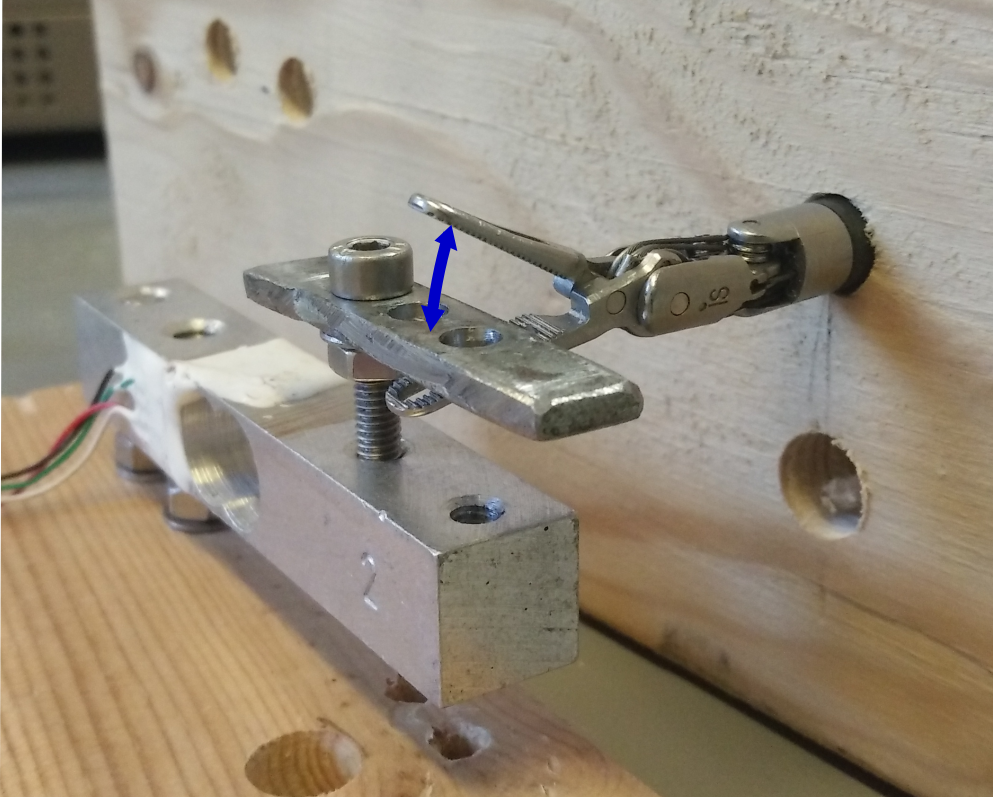
\includegraphics[width=\linewidth,height=5.4cm]{clamp_mes.png}
		\caption{Upper clamp which is allowed to add or release force applied to the load-cell.}
		\label{fig:one_clamp}
	\end{subfigure}
	% \begin{subfigure}{.32\textwidth}
	% 	\centering
	% 	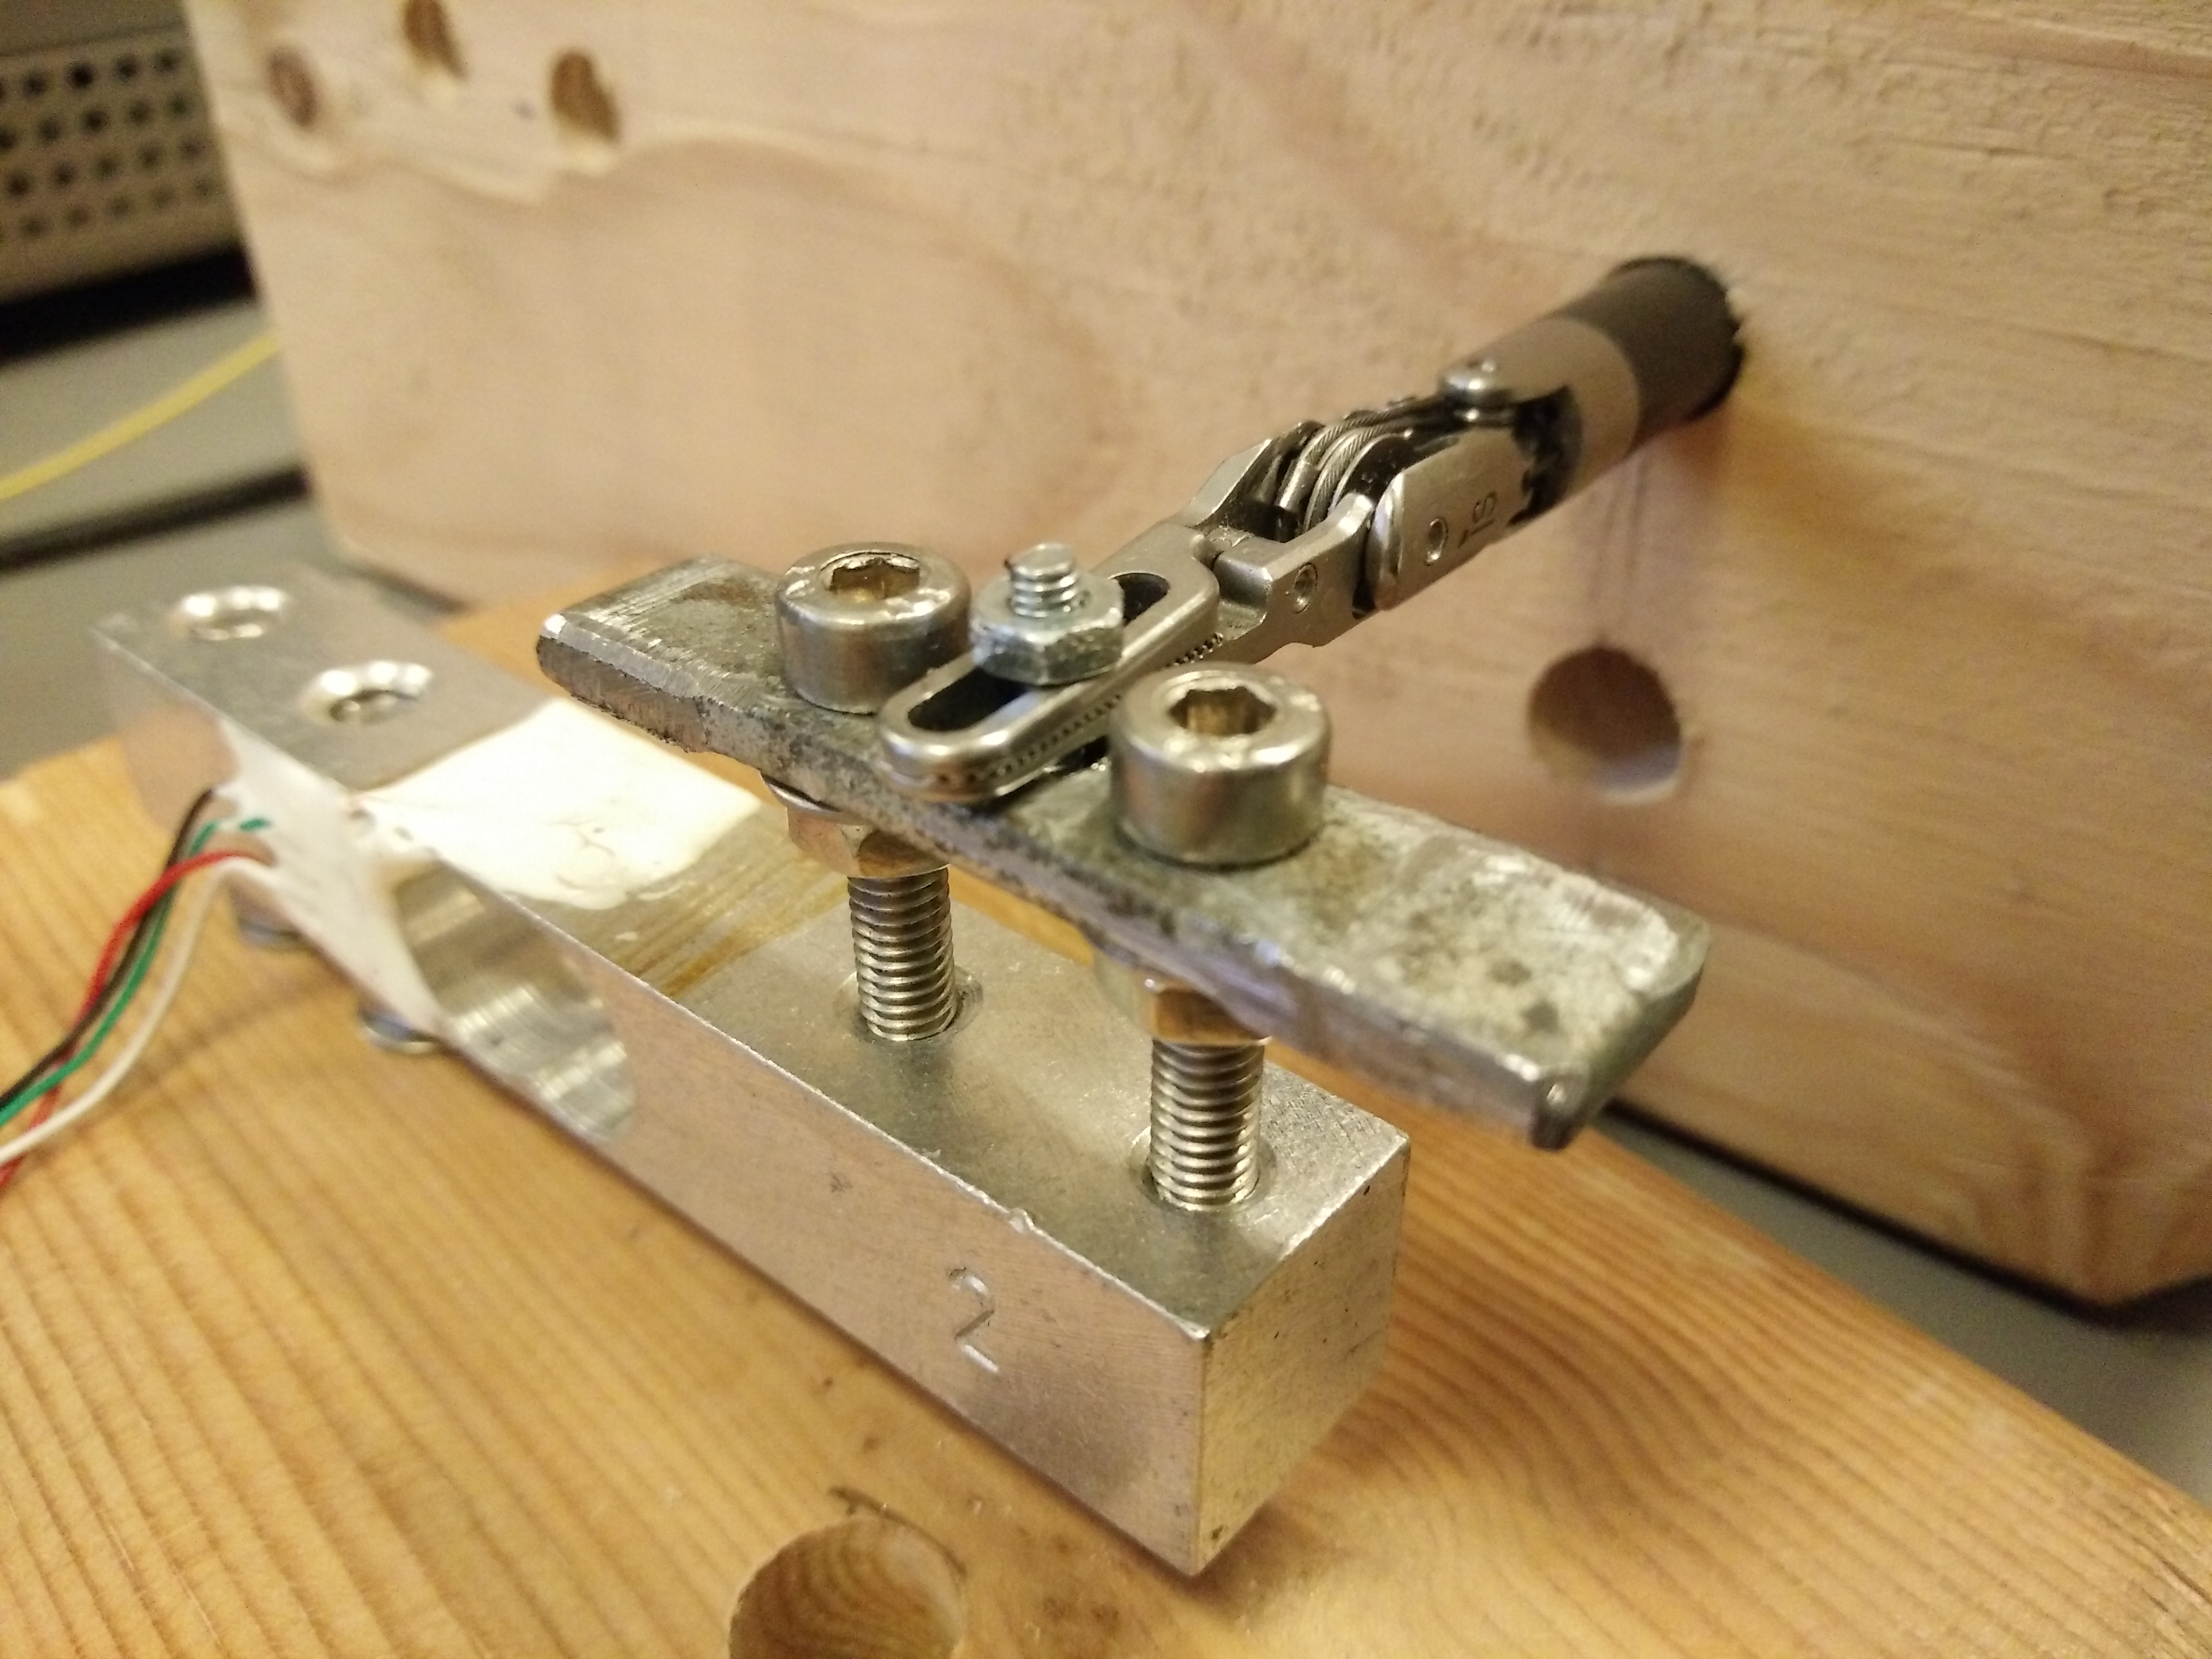
\includegraphics[width=\linewidth]{Two_clamp.jpg}
	% 	\caption{The clamps are put together and connected to the load-cell such that the pull/push force can be measured.}
	% 	\label{fig:two_clamp}
	% \end{subfigure}
	\begin{subfigure}{.48\textwidth}
		\centering
		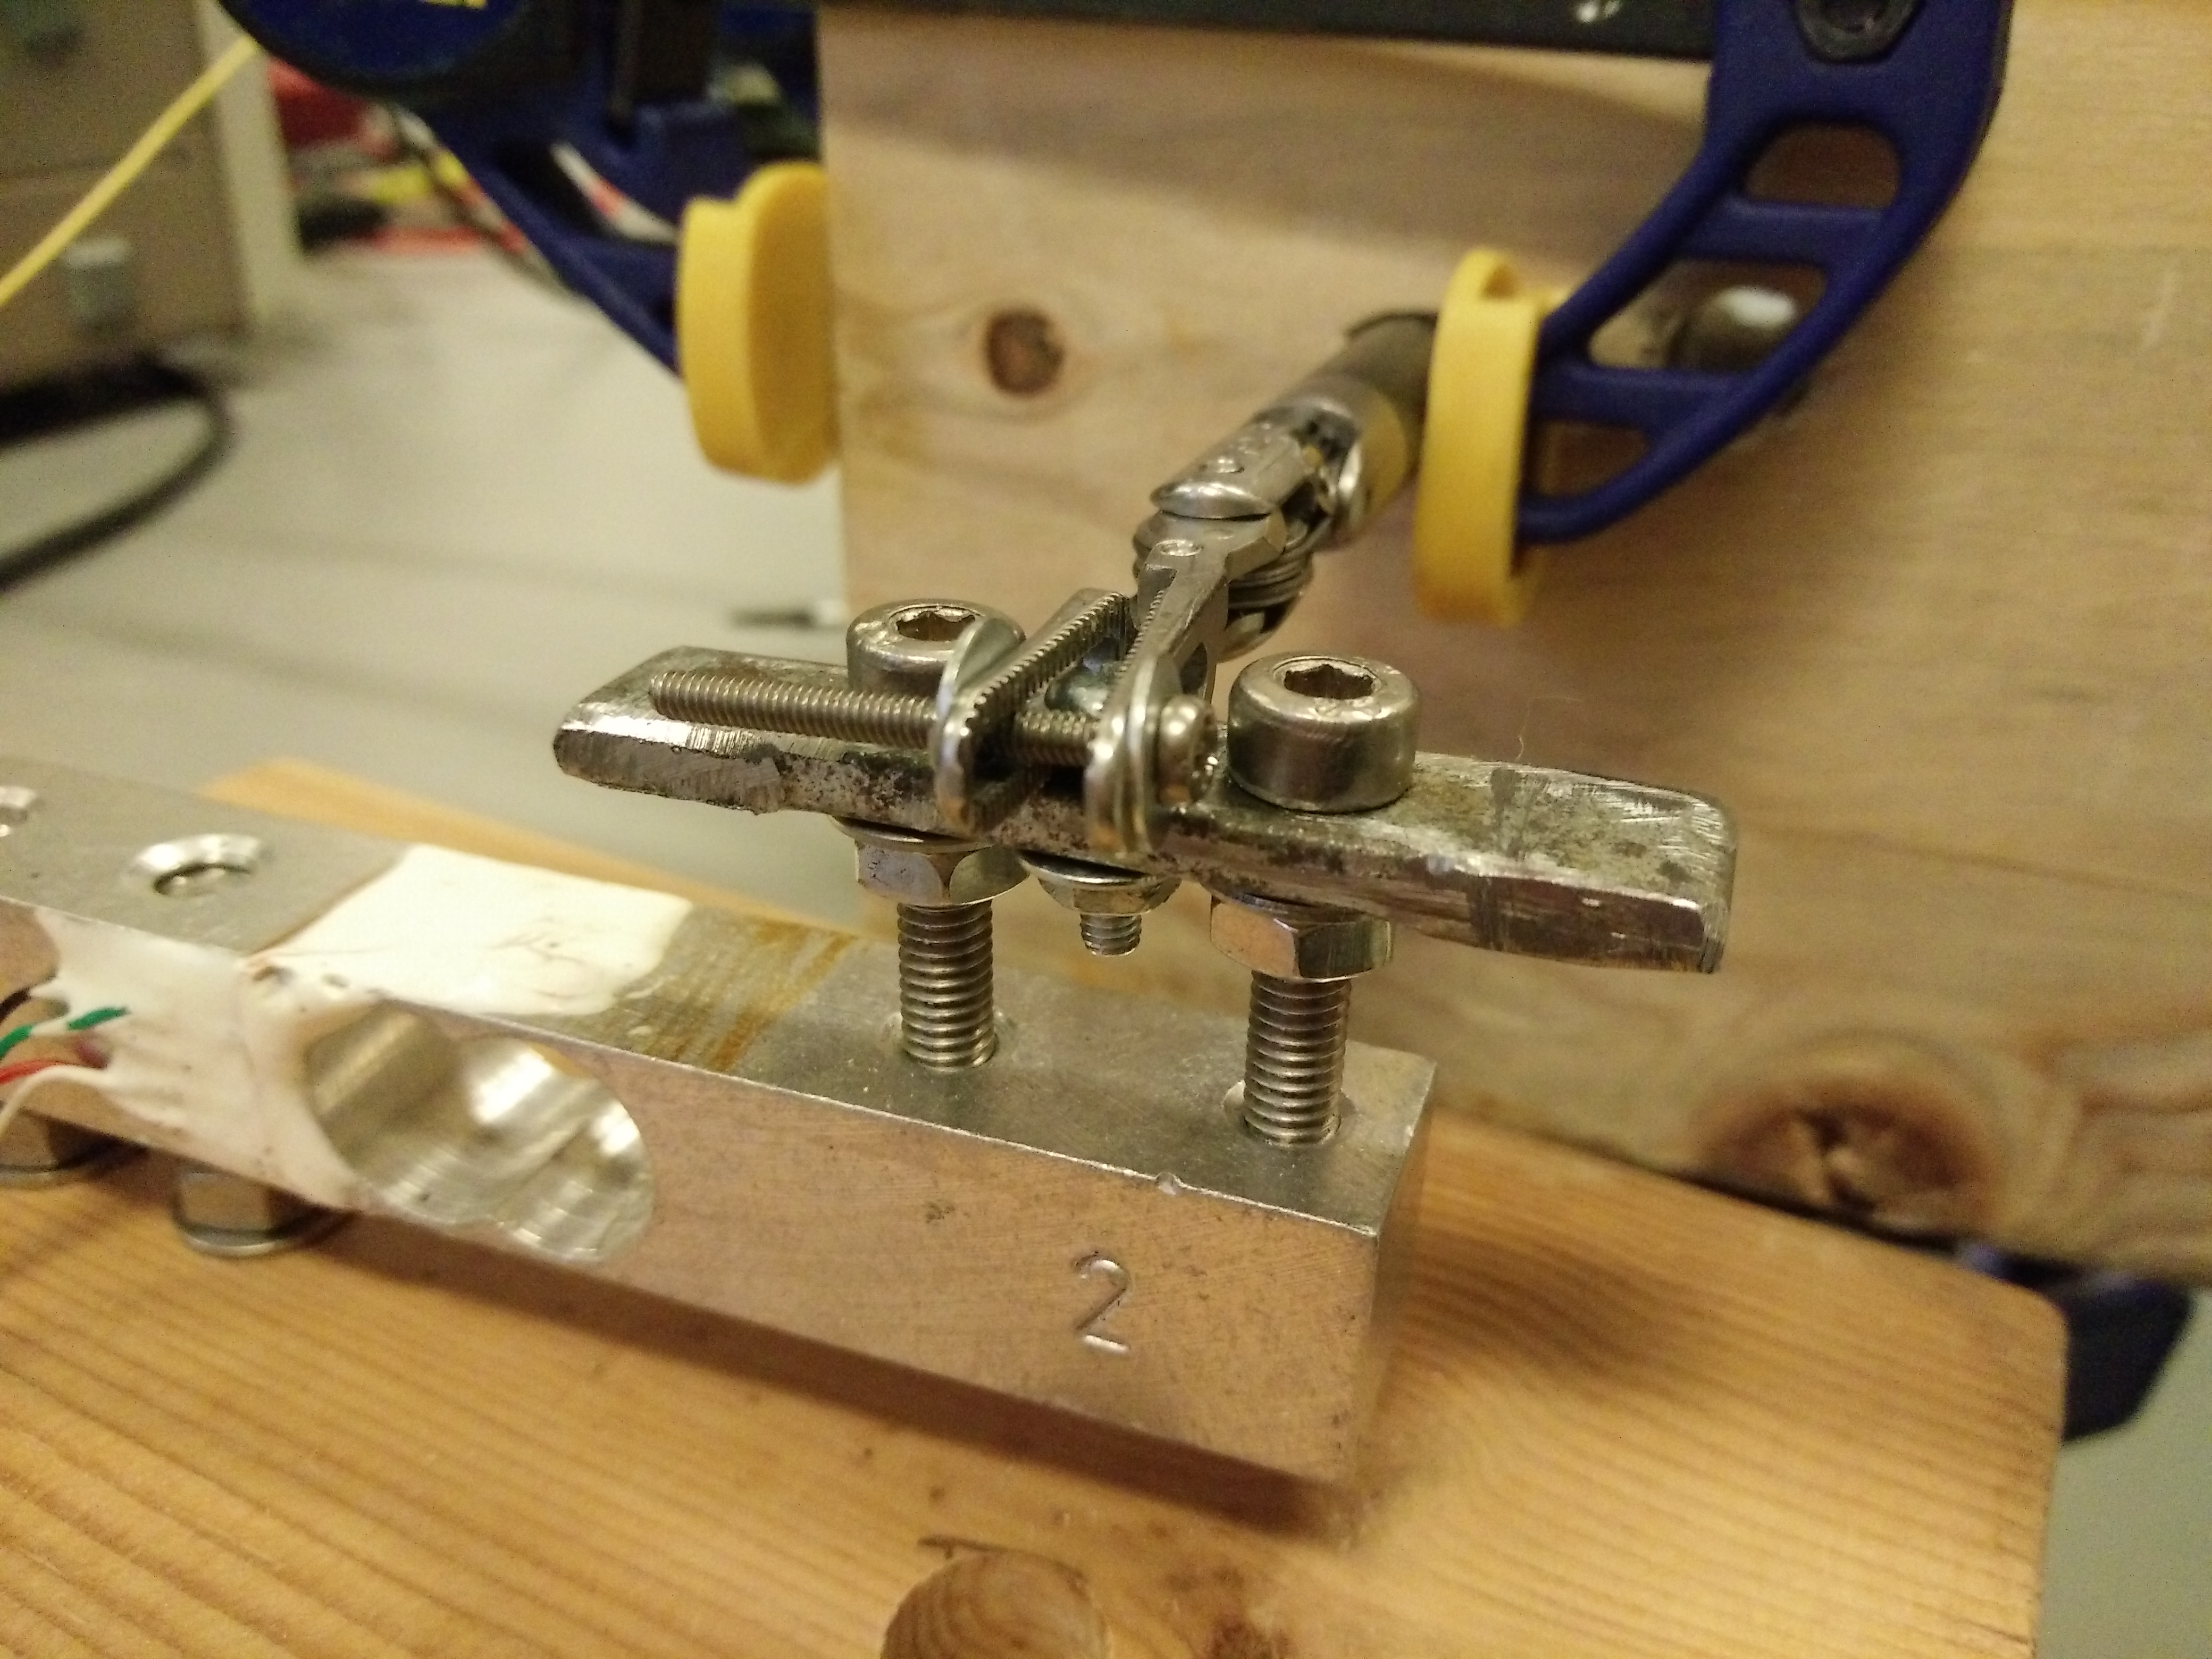
\includegraphics[width=\linewidth]{Pitch_clamp.jpg}
		\caption{The end-effectors two clamps are attached to the load-cell, such that the pitch force can be measured.}
		\label{fig:pitch_force}
	\end{subfigure}
\caption{Attachments between the end-effector and the load-cell used for force measurements}
\label{fig:Overview_endowrist_attachment}
\end{figure}

\subsection*{Electrical circuit}
For making the force measurement for the EndoWrist a simple hardware construction was build. A simple block diagram of setup can be seen on \figref{fig:arduino_loadcell}

\begin{figure}[H]
\centering
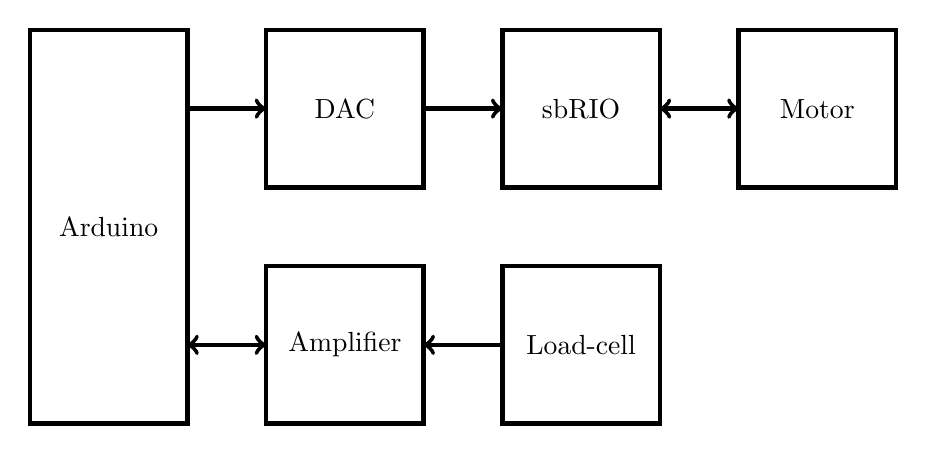
\begin{tikzpicture}%[every node/.style={draw,outer sep=0pt,thick}]

\draw [ultra thick] (0,0) rectangle (2,2);
\node at (1,1) {Load-cell};
\draw [->,ultra thick] (0,1) -- (-1,1);

\draw [ultra thick] (-3,0) rectangle (-1,2);
\node at (-2,1) {Amplifier};
\draw [<->,ultra thick] (-3,1) -- (-4,1);

\draw [ultra thick] (3,3) rectangle (5,5);
\node at (4,4) {Motor};
\draw [<-,ultra thick] (2,4) -- (3,4);
\draw [->,ultra thick] (2,4) -- (3,4);

\draw [ultra thick] (0,3) rectangle (2,5);
\node at (1,4) {sbRIO};
\draw [<-,ultra thick] (0,4) -- (-1,4);

\draw [ultra thick] (-3,3) rectangle (-1,5);
\node at (-2,4) {DAC};
\draw [<-,ultra thick] (-3,4) -- (-4,4);

\draw [ultra thick] (-6,0) rectangle (-4,5);
\node at (-5,2.5) {Arduino};

\end{tikzpicture}
\caption{Diagram of the test setup for the force measurements.}
\label{fig:arduino_loadcell}
\end{figure}

The load-cell's output is amplified and send to an Arduino which calculate the force applied to the load-cell. The force is then translated to a corresponding voltage output, $mV\cdot\frac{g}{4\cdot mV}$. Since the Arduino does not have a digital to analog converter (DAC), the voltage is translated to a binary code and send to a "Max531 DAC" through a serial peripheral interface (SPI). The voltage output from the DAC is read at the sbRIO board which also samples the current send to the motor, motor position and time stamps.

As explained, an Arduino is used for the translation of force applied to the load-cell. This was done since a library for the HX711 amplifier was made for the Arduino IDE\cite{Git_HX711}. This library included features such as calibration, reset and averaging of the load-cell. 



%\todo{not in use}
\subsection{Grip force} % \label{app:...}

This test uses the test setup seen on \figref{fig:one_clamp}. The positive force is defined as downwards direction on the load-cell, see \figref{fig:mes_up_down1}.

\begin{figure}[H]
	\centering
	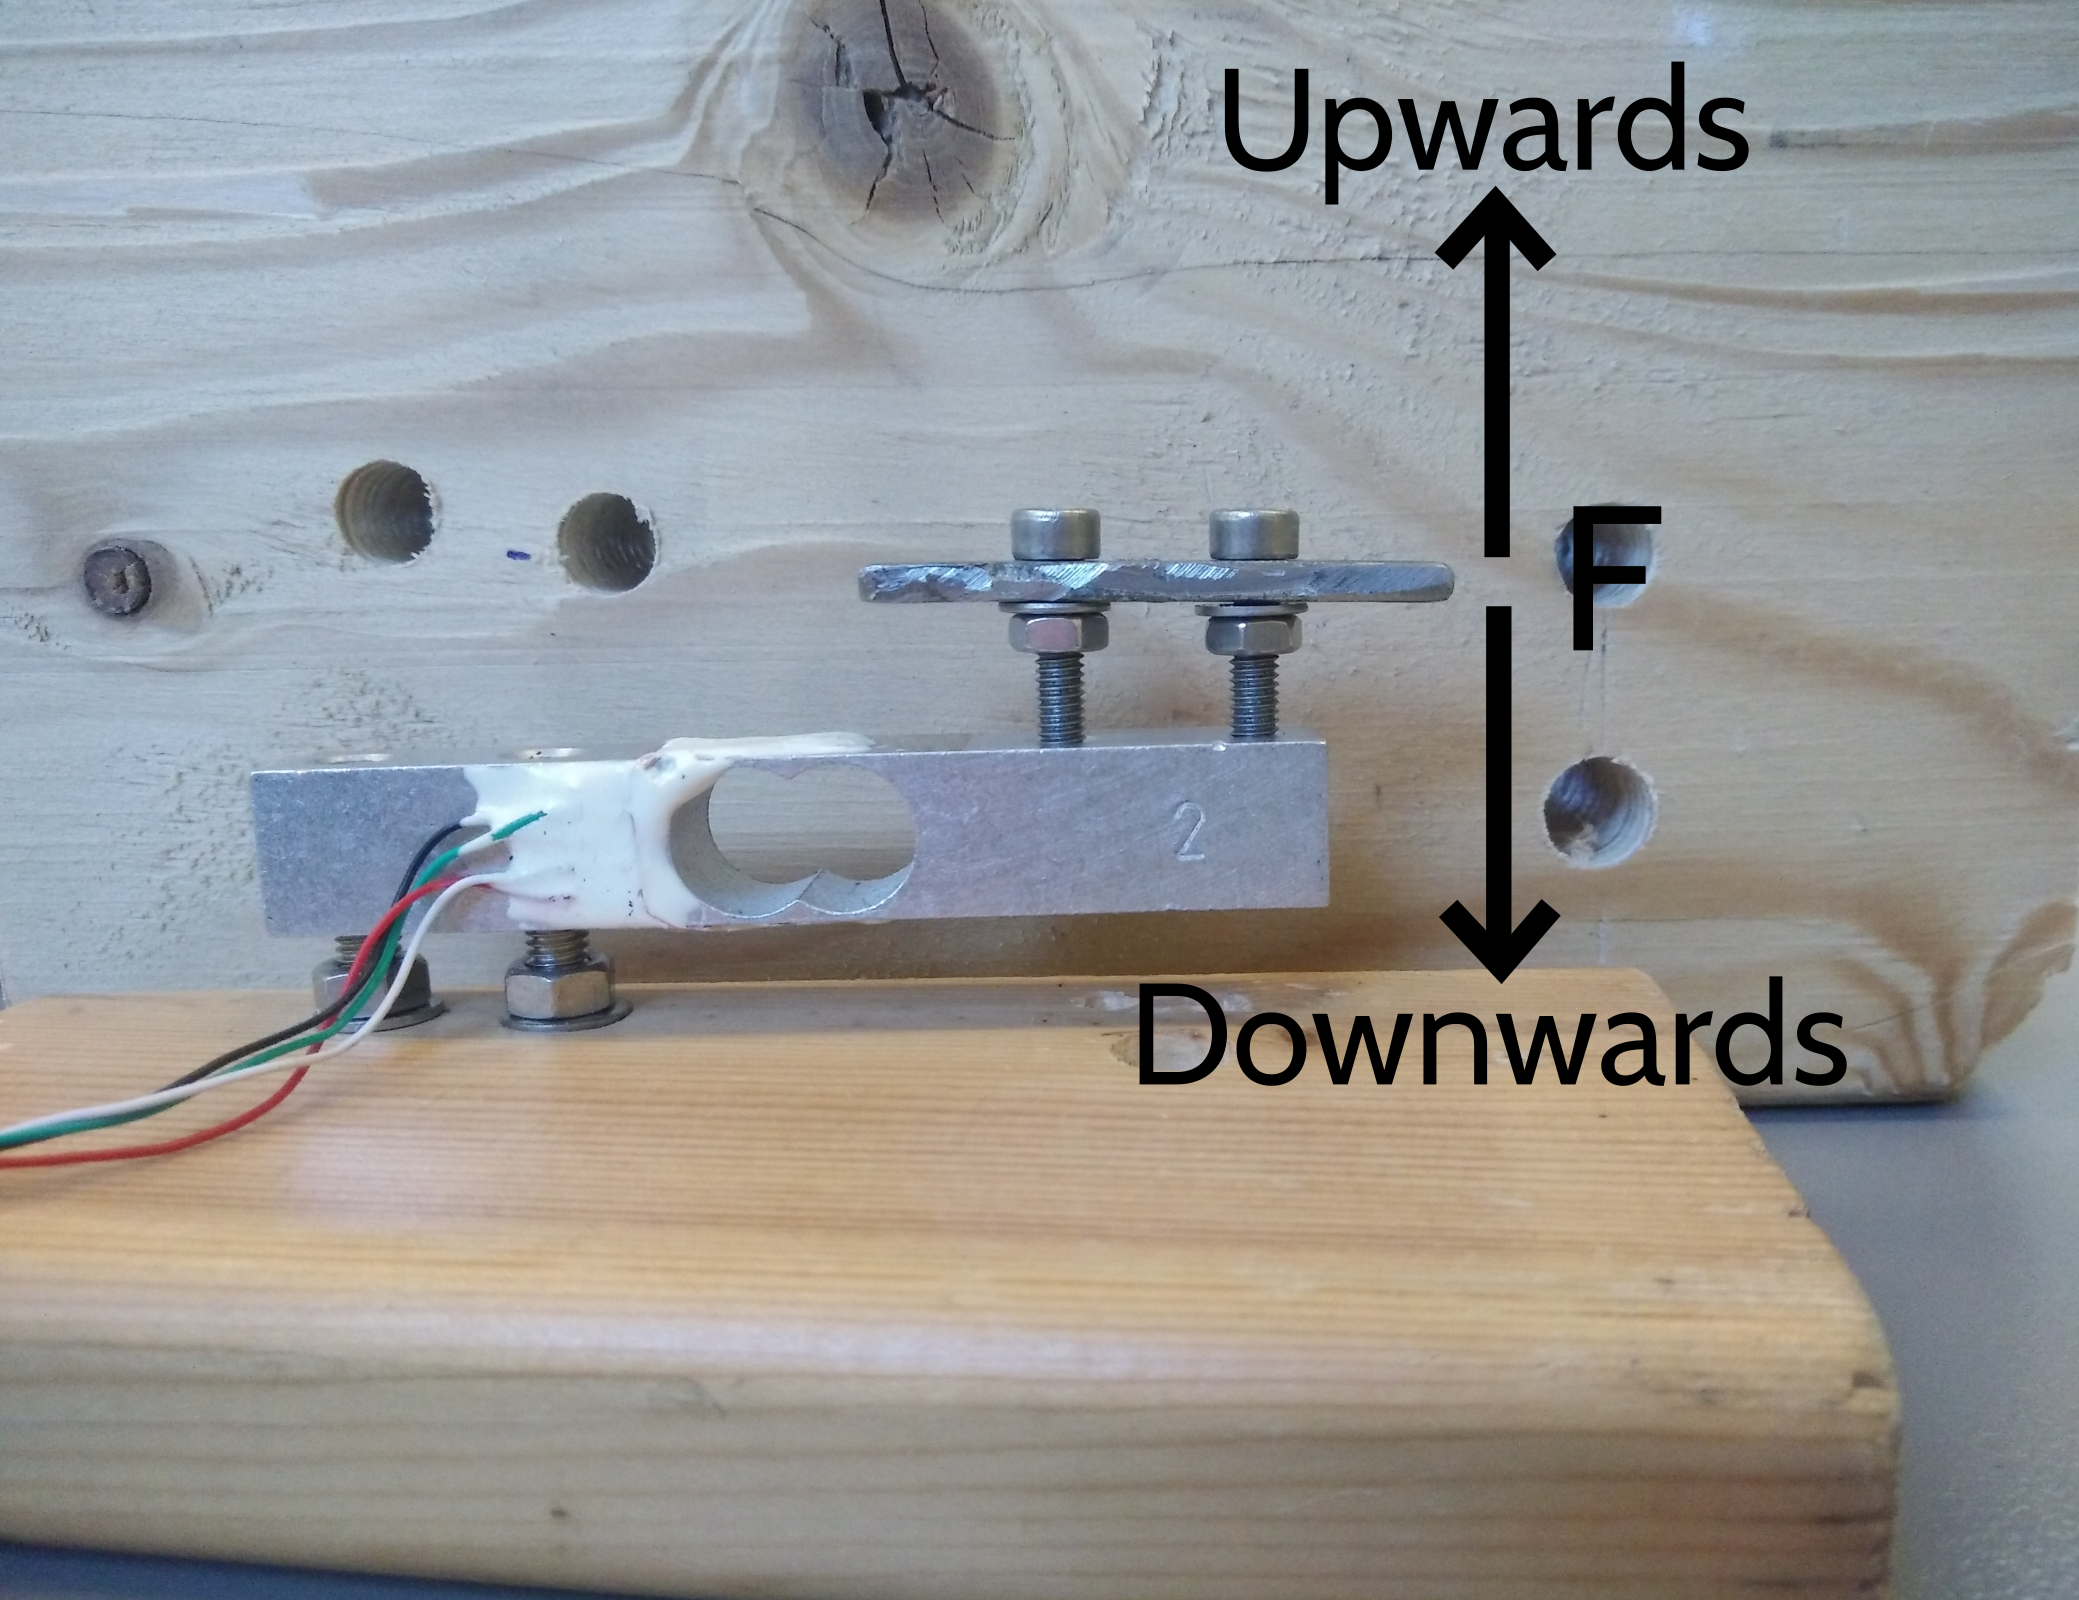
\includegraphics[width=0.4\linewidth]{load_cell_mes.png}
	\caption{Load-cell with defined upwards- downwars force.}
	\label{fig:mes_up_down1}
\end{figure}


\subsection*{Test equipment:}
\begin{itemize}
\item Endowrist model 420093 (AAU number: \#4).
\item Maxon 110160 motor with attached Maxon gearhead 110356 and Maxon encoder 201937.
\item Load cell rate for 1 kg of force \cite{Load_cell_1kg}.
\item HX711 - Load cell amplifier \cite{HX711}.
\item Arduino uno with Max351 DAC.
\item sbRIO board.
\end{itemize}

\subsection*{Procedure:}
The following procedures was made for the dynamic measurements of one clamp on the EndoWrist.

\begin{enumerate}
\item One clamp is enabled and put above the load-cell as seen on \figref{fig:one_clamp}.
\item The scale is set to zero.
\item Alternating setpoints are send to the motor controlling the upper clamp in a triangular wave.
\item Current, force and velocity is sampled.
\end{enumerate}
Each test is running for a short period of time, since the input setpoints are periodic. This test was done 11 times.

\subsection*{Measuring data:}
The data form one measurement is shown on \figref{yaw_mes123}.
\begin{figure}[H]
\centering
\input{Data/Measurement/EndoWrist_Measurements/Force/yaw_mes}
\caption{One set of data that shows the force, current and velocity. The interval between the red lines shows one period of contact with the load cell and the green is the release of the force applied.}
\label{yaw_mes123}
\end{figure}

%\figref{endo_force_mes}. 
%\eqref{eq:linear_force_endo}.

% \begin{equation}
% \text{y} = 0.0028 \cdot \text{x} -0.8259 
% \label{eq:linear_force_endo}
% \end{equation} 


\subsection*{Results:}
From \figref{yaw_mes123}, one of the measurements for the grip force estimation is shown. The first red line marks one of the starting periods, where contact between the clamp and the load-cell is happening. It can be seen that a current increase is happening in when the load-cell is applied force. When the current decreases the force is kept until the sign on the current has changed and force is applied in an upwards direction of the clamp. 


%It can be seen from the graph on \figref{endo_force_mes} that the force on the end-effector is highly nonlinear. The friction from the gearing and the Endowrist does that the force first has an exponential growth at the start. Around the 800 mA and 1200 mA step it can be seen that a drop in force is happening. What causes this drop is not identified but it can be seen that it appears for all the data sequences. \todor{better explanation?}


%% This file was created by matlab2tikz.
%
%The latest updates can be retrieved from
%  http://www.mathworks.com/matlabcentral/fileexchange/22022-matlab2tikz-matlab2tikz
%where you can also make suggestions and rate matlab2tikz.
%
\definecolor{mycolor1}{rgb}{0.00000,0.44700,0.74100}%
\definecolor{mycolor2}{rgb}{0.85000,0.32500,0.09800}%
%
\begin{figure}[h]
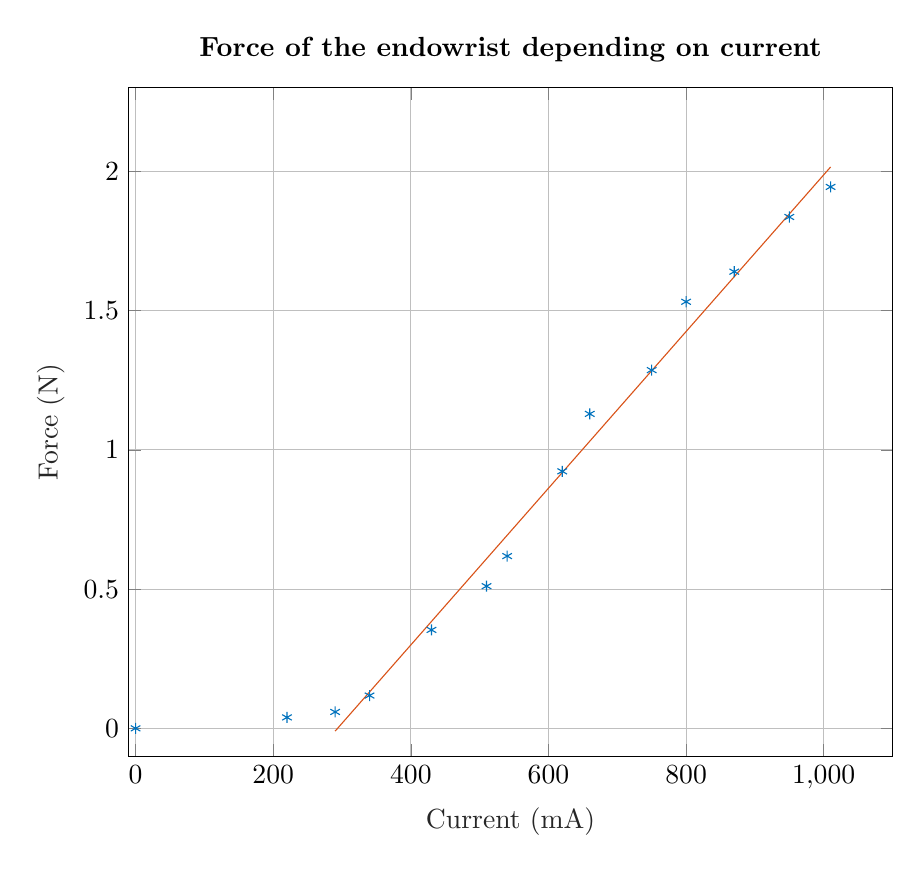
\begin{tikzpicture}

\begin{axis}[%
width=0.8\columnwidth,%7.484in,
height=0.7\columnwidth,%8.26in,
at={(0.758in,0.481in)},
scale only axis,
xmin=-10,
xmax=1100,
xlabel style={font=\color{white!15!black}},
xlabel={Current (mA)},
ymin=-0.1,
ymax=2.3,
ylabel style={font=\color{white!15!black}},
ylabel={Force (N)},
axis background/.style={fill=white},
title style={font=\bfseries},
title={Force of the endowrist depending on current},
xmajorgrids,
ymajorgrids
]
\addplot [color=mycolor1, draw=none, mark=asterisk, mark options={solid, mycolor1}, forget plot]
  table[row sep=crcr]{%
0	0\\
220	0.03928\\
290	0.05892\\
340	0.11784\\
430	0.35352\\
510	0.51064\\
540	0.61866\\
620	0.92308\\
660	1.1293\\
750	1.28642\\
800	1.53192\\
870	1.63994\\
950	1.83634\\
1010	1.94436\\
};
\addplot [color=mycolor2, forget plot]
  table[row sep=crcr]{%
290	-0.00996204344902341\\
340	0.130719594329395\\
430	0.383946542330548\\
510	0.609037162776017\\
540	0.693446145443068\\
620	0.918536765888537\\
660	1.03108207611127\\
750	1.28430902411242\\
800	1.42499066189084\\
870	1.62194495478063\\
950	1.8470355752261\\
1010	2.0158535405602\\
};
\end{axis}
\end{tikzpicture}%
\caption{The force measurements from the end-effector}
\label{endo_force_mes}
\end{figure}

\subsection*{Uncertainties of measurement:}
\begin{itemize}
\item Not 100 \% orthogonal force to the load cell.
\item Input/Output impedance of sensors have a $\pm 10 \%$ tolerance.
\item Movement of test setup when force is generated.
\item The pitch joint of the EndoWrist had a tendency to bend when high force was applied which change the force direction. 
\end{itemize}

\subsection*{Conclusion:}
It can be seen that there is a high friction in mechanical part that handles the clamp. Due to this friction, the tool is able to withhold a force when the current is decreasing.
%\todo{not in use}
%\subsection{Clamp two} % \label{app:...}
This test uses the test setup seen on \figref{fig:one_clamp}. A positive force for the clamps are defined as an inwards force.

\subsection*{Test equipment:}
\begin{itemize}
\item Endowrist model 420093 (AAU number: \#4).
\item Maxon 110160 motor with attached Maxon gearhead 110356 and Maxon encoder 201937.
\item Load cell rate for 1 kg of force \cite{Load_cell_1kg}.
\item HX711 - Load cell amplifier \cite{HX711}.
\item Arduino uno with Max351 DAC.
\item sbRIO board.
\end{itemize}

\subsection*{Procedure:}
The following procedures was made for the force estimation of clamp 2 on the EndoWrist. 
Inwards force:
\begin{enumerate}
\item One clamp of the end-effector is attached perpendicular to the load cell. 
\item The scale is set to zero.
\item Current is applied to the motor which control the clamp attached to the load-cell and the force is measured (inwards direction).
\item Current is increased in steps until 1200 mA is applied.
\end{enumerate}
Step two to four is repeated eight times, where the current and force is measured in respect to each other. 

Outwards force:
\begin{enumerate}
\item One clamp of the end-effector is attached perpendicular to the load cell. 
\item The scale is set to zero.
\item Current is applied to the motor which control the clamp attached to the load-cell and the force is measured (outwards direction).
\item Current is increased in steps until 1200 mA is applied.
\end{enumerate}
Step two to four is repeated eight times, where the current and force is measured in respect to each other. 

\subsection*{Measuring data:}
The data from six of the measurements can be seen on \figref{fig:2_clamp_in} and \figref{fig:2_clamp_out}.

\input{Data/Measurement/EndoWrist_Measurements/Force/2_One_clamp_in}

\input{Data/Measurement/EndoWrist_Measurements/Force/2_One_clamp_out}
%\figref{endo_force_mes}. 
%\eqref{eq:linear_force_endo}.

% \begin{equation}
% \text{y} = 0.0028 \cdot \text{x} -0.8259 
% \label{eq:linear_force_endo}
% \end{equation} 

\subsection*{Results:}
From \figref{fig:2_clamp_in} and \figref{fig:2_clamp_out} six different measurements can be seen for clamp two of the EndoWrist.
It can be seen due to static friction from the motor, gearing and the EndoWrist, that a current of approx 500 mA for the inwards and outwards force is needed before movement. It can also be seen that there is different growth in force, in respect to the current, for the different measurements. This is probably because of the elasticity of the tool. Depending of the start position of the tool, the wire can either be in a relaxed or stressed state. If the wire is in a relaxed state the motor can rotate a littel and build up a small inertia to help overcome the friction of the EndoWrist. It can be seen on each measurement, that there is a sharp current decrease. This is because of a safety feature in the Escon motor controller setup, where it needs the nominal current for the motor. The motor controller can handle a current peak for a certain amount of time and then it will limit the current to the nominal. It should be noted when the current drops the maximum force is still applied to the load-cell. This is probably due to the friction of the tool. When the maximum force is applied and the current drops, the friction will help keeping the force. At \figref{fig:2_clamp_out} it can be seen from 8 - 12 seconds that a force is increasing and decreasing. This is due to the construction of the test setup. If the EndoWrist is not supported at correctly at the end, the pitch had a tendency to bend a little, which alter the force direction applied to the load-cell.

%It can be seen from the graph on \figref{endo_force_mes} that the force on the end-effector is highly nonlinear. The friction from the gearing and the Endowrist does that the force first has an exponential growth at the start. Around the 800 mA and 1200 mA step it can be seen that a drop in force is happening. What causes this drop is not identified but it can be seen that it appears for all the data sequences. \todor{better explanation?}


%% This file was created by matlab2tikz.
%
%The latest updates can be retrieved from
%  http://www.mathworks.com/matlabcentral/fileexchange/22022-matlab2tikz-matlab2tikz
%where you can also make suggestions and rate matlab2tikz.
%
\definecolor{mycolor1}{rgb}{0.00000,0.44700,0.74100}%
\definecolor{mycolor2}{rgb}{0.85000,0.32500,0.09800}%
%
\begin{figure}[h]
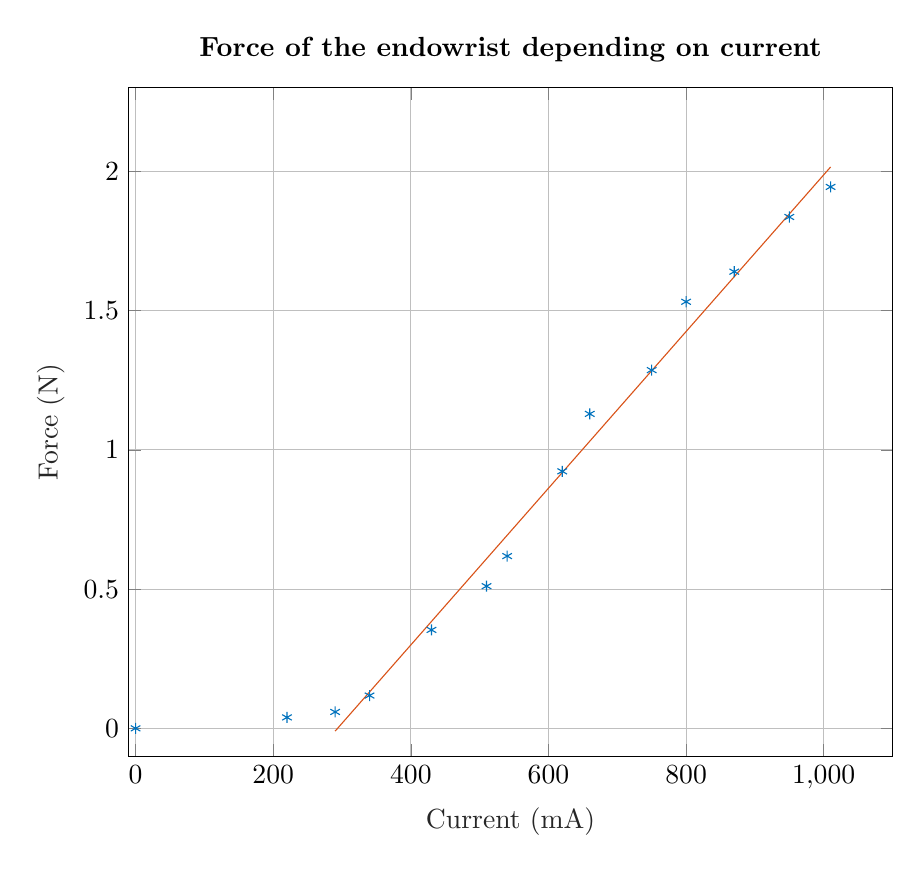
\begin{tikzpicture}

\begin{axis}[%
width=0.8\columnwidth,%7.484in,
height=0.7\columnwidth,%8.26in,
at={(0.758in,0.481in)},
scale only axis,
xmin=-10,
xmax=1100,
xlabel style={font=\color{white!15!black}},
xlabel={Current (mA)},
ymin=-0.1,
ymax=2.3,
ylabel style={font=\color{white!15!black}},
ylabel={Force (N)},
axis background/.style={fill=white},
title style={font=\bfseries},
title={Force of the endowrist depending on current},
xmajorgrids,
ymajorgrids
]
\addplot [color=mycolor1, draw=none, mark=asterisk, mark options={solid, mycolor1}, forget plot]
  table[row sep=crcr]{%
0	0\\
220	0.03928\\
290	0.05892\\
340	0.11784\\
430	0.35352\\
510	0.51064\\
540	0.61866\\
620	0.92308\\
660	1.1293\\
750	1.28642\\
800	1.53192\\
870	1.63994\\
950	1.83634\\
1010	1.94436\\
};
\addplot [color=mycolor2, forget plot]
  table[row sep=crcr]{%
290	-0.00996204344902341\\
340	0.130719594329395\\
430	0.383946542330548\\
510	0.609037162776017\\
540	0.693446145443068\\
620	0.918536765888537\\
660	1.03108207611127\\
750	1.28430902411242\\
800	1.42499066189084\\
870	1.62194495478063\\
950	1.8470355752261\\
1010	2.0158535405602\\
};
\end{axis}
\end{tikzpicture}%
\caption{The force measurements from the end-effector}
\label{endo_force_mes}
\end{figure}

\subsection*{Uncertainties of measurement:}
\begin{itemize}
\item Not 100 \% orthogonal force to the load cell.
\item Input/Output impedance of sensors have a $\pm 10 \%$ tolerance.
\item Movement of test setup when force is generated.
\item The pitch joint of the EndoWrist had a tendency to bend when high force was applied which change the force direction.
\end{itemize}

\subsection*{Conclusion:}
\todo{conclusion}

%\subsection{One clamp push} % \label{app:...}
This test uses the test setup seen on \figref{fig:one_clamp}.

\subsection*{Test equipment:}
\begin{itemize}
\item Endowrist model 420093 (AAU number: \#4).
\item Maxon 110160 motor with attached Maxon gearhead 110356 and Maxon encoder 201937.
\item Load cell rate for 1 kg of force \cite{Load_cell_1kg}.
\item HX711 - Load cell amplifier \cite{HX711}
\end{itemize}

\subsection*{Procedure:}
The following procedure was made for the force estimation:
\begin{enumerate}
\item One clamp of the end-effector is attached perpendicular to the load cell. 
\item The scale is set to zero.
\item Current is applied to the motor which control the clamp attached to the load-cell and the force is measured (upwards direction).
\item Current is increased in steps until 1200 mA is applied.
\end{enumerate}
Step two to four is repeated ten times, where the current and force is measured in respect to each other. 


\subsection*{Measuring data:}
The data from the measurements can be seen on \todo{Picture}%\figref{endo_force_mes}. 
%\eqref{eq:linear_force_endo}.

% \begin{equation}
% \text{y} = 0.0028 \cdot \text{x} -0.8259 
% \label{eq:linear_force_endo}
% \end{equation} 



\subsection*{Results:}
\todo{result}
%It can be seen from the graph on \figref{endo_force_mes} that the force on the end-effector is highly nonlinear. The friction from the gearing and the Endowrist does that the force first has an exponential growth at the start. Around the 800 mA and 1200 mA step it can be seen that a drop in force is happening. What causes this drop is not identified but it can be seen that it appears for all the data sequences. \todor{better explanation?}


%% This file was created by matlab2tikz.
%
%The latest updates can be retrieved from
%  http://www.mathworks.com/matlabcentral/fileexchange/22022-matlab2tikz-matlab2tikz
%where you can also make suggestions and rate matlab2tikz.
%
\definecolor{mycolor1}{rgb}{0.00000,0.44700,0.74100}%
\definecolor{mycolor2}{rgb}{0.85000,0.32500,0.09800}%
%
\begin{figure}[h]
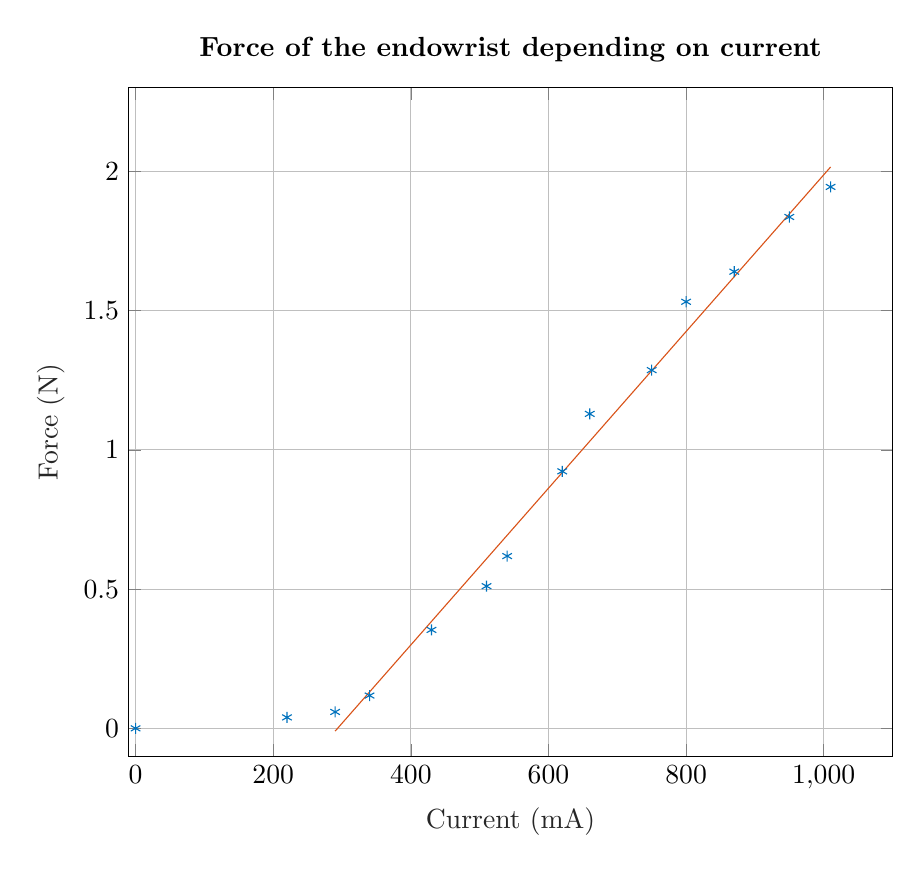
\begin{tikzpicture}

\begin{axis}[%
width=0.8\columnwidth,%7.484in,
height=0.7\columnwidth,%8.26in,
at={(0.758in,0.481in)},
scale only axis,
xmin=-10,
xmax=1100,
xlabel style={font=\color{white!15!black}},
xlabel={Current (mA)},
ymin=-0.1,
ymax=2.3,
ylabel style={font=\color{white!15!black}},
ylabel={Force (N)},
axis background/.style={fill=white},
title style={font=\bfseries},
title={Force of the endowrist depending on current},
xmajorgrids,
ymajorgrids
]
\addplot [color=mycolor1, draw=none, mark=asterisk, mark options={solid, mycolor1}, forget plot]
  table[row sep=crcr]{%
0	0\\
220	0.03928\\
290	0.05892\\
340	0.11784\\
430	0.35352\\
510	0.51064\\
540	0.61866\\
620	0.92308\\
660	1.1293\\
750	1.28642\\
800	1.53192\\
870	1.63994\\
950	1.83634\\
1010	1.94436\\
};
\addplot [color=mycolor2, forget plot]
  table[row sep=crcr]{%
290	-0.00996204344902341\\
340	0.130719594329395\\
430	0.383946542330548\\
510	0.609037162776017\\
540	0.693446145443068\\
620	0.918536765888537\\
660	1.03108207611127\\
750	1.28430902411242\\
800	1.42499066189084\\
870	1.62194495478063\\
950	1.8470355752261\\
1010	2.0158535405602\\
};
\end{axis}
\end{tikzpicture}%
\caption{The force measurements from the end-effector}
\label{endo_force_mes}
\end{figure}

\subsection*{Uncertainties of measurement:}
\begin{itemize}
\item Not 100 \% orthogonal force to the load cell.
\item Input/Output impedance of sensors have a $\pm 10 \%$ tolerance.
\item Movement of test setup when force is generated.
\end{itemize}

\subsection*{Conclusion:}
\todo{conclusion}
%\todo{not in use}
%\subsection{Two clamp pull} % \label{app:...}
This test uses the test setup seen on \figref{fig:two_clamp}.


\subsection*{Test equipment:}
\begin{itemize}
\item Endowrist model 420093 (AAU number: \#4).
\item Maxon 110160 motor with attached Maxon gearhead 110356 and Maxon encoder 201937.
\item Load cell rate for 1 kg of force \cite{Load_cell_1kg}.
\item HX711 - Load cell amplifier \cite{HX711}.
\item Arduino uno with Max351 DAC.
\item sbRIO board.
\end{itemize}


\subsection*{Procedure:}
The following procedure was made for the push force measurements:
\begin{enumerate}
\item The two end-effector clamps are attached perpendicular to the load cell. 
\item The scale is reset to zero.
\item Current is applied to the motors which control the clamps of the end-effector and the force is measured (downwards direction).
\item Current is increased in steps until 1200 mA is applied.
\end{enumerate}
Step two to four is repeated ten times, where the current and force is measured in respect to each other. 

\subsection*{Measuring data:}
The data from the measurements can be seen on \todo{Picture}%\figref{endo_force_mes}. 
%\eqref{eq:linear_force_endo}.

% \begin{equation}
% \text{y} = 0.0028 \cdot \text{x} -0.8259 
% \label{eq:linear_force_endo}
% \end{equation} 



\subsection*{Results:}
\todo{result}
%It can be seen from the graph on \figref{endo_force_mes} that the force on the end-effector is highly nonlinear. The friction from the gearing and the Endowrist does that the force first has an exponential growth at the start. Around the 800 mA and 1200 mA step it can be seen that a drop in force is happening. What causes this drop is not identified but it can be seen that it appears for all the data sequences. \todor{better explanation?}


%% This file was created by matlab2tikz.
%
%The latest updates can be retrieved from
%  http://www.mathworks.com/matlabcentral/fileexchange/22022-matlab2tikz-matlab2tikz
%where you can also make suggestions and rate matlab2tikz.
%
\definecolor{mycolor1}{rgb}{0.00000,0.44700,0.74100}%
\definecolor{mycolor2}{rgb}{0.85000,0.32500,0.09800}%
%
\begin{figure}[h]
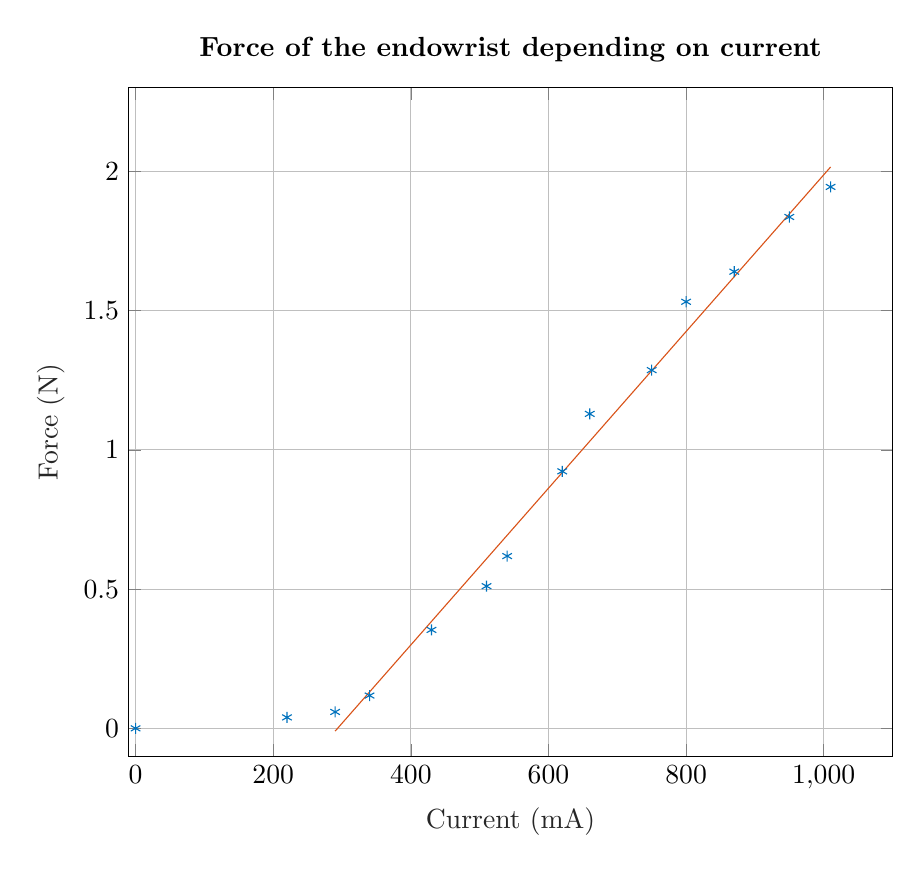
\begin{tikzpicture}

\begin{axis}[%
width=0.8\columnwidth,%7.484in,
height=0.7\columnwidth,%8.26in,
at={(0.758in,0.481in)},
scale only axis,
xmin=-10,
xmax=1100,
xlabel style={font=\color{white!15!black}},
xlabel={Current (mA)},
ymin=-0.1,
ymax=2.3,
ylabel style={font=\color{white!15!black}},
ylabel={Force (N)},
axis background/.style={fill=white},
title style={font=\bfseries},
title={Force of the endowrist depending on current},
xmajorgrids,
ymajorgrids
]
\addplot [color=mycolor1, draw=none, mark=asterisk, mark options={solid, mycolor1}, forget plot]
  table[row sep=crcr]{%
0	0\\
220	0.03928\\
290	0.05892\\
340	0.11784\\
430	0.35352\\
510	0.51064\\
540	0.61866\\
620	0.92308\\
660	1.1293\\
750	1.28642\\
800	1.53192\\
870	1.63994\\
950	1.83634\\
1010	1.94436\\
};
\addplot [color=mycolor2, forget plot]
  table[row sep=crcr]{%
290	-0.00996204344902341\\
340	0.130719594329395\\
430	0.383946542330548\\
510	0.609037162776017\\
540	0.693446145443068\\
620	0.918536765888537\\
660	1.03108207611127\\
750	1.28430902411242\\
800	1.42499066189084\\
870	1.62194495478063\\
950	1.8470355752261\\
1010	2.0158535405602\\
};
\end{axis}
\end{tikzpicture}%
\caption{The force measurements from the end-effector}
\label{endo_force_mes}
\end{figure}

\subsection*{Uncertainties of measurement:}
\begin{itemize}
\item Not 100 \% orthogonal force to the load cell.
\item Input/Output impedance of sensors have a $\pm 10 \%$ tolerance.
\item Movement of test setup when force is generated.
\end{itemize}

\subsection*{Conclusion:}
\todo{conclusion}
%\todo{not in use}
%\subsection{Two clamp push} % \label{app:...}
This test uses the test setup seen on \figref{fig:two_clamp}.

\subsection*{Test equipment:}
\begin{itemize}
\item Endowrist model 420093 (AAU number: \#4).
\item Maxon 110160 motor with attached Maxon gearhead 110356 and Maxon encoder 201937.
\item Load cell rate for 1 kg of force \cite{Load_cell_1kg}.
\item HX711 - Load cell amplifier \cite{HX711}
\end{itemize}

\subsection*{Procedure:}
The following procedure was made for the push force measurements:
\begin{enumerate}
\item The two end-effector clamps are attached perpendicular to the load cell. 
\item The scale is reset to zero.
\item Current is applied to the motors which control the clamps of the end-effector and the force is measured (upwards direction).
\item Current is increased in steps until 1200 mA is applied.
\end{enumerate}
Step two to four is repeated ten times, where the current and force is measured in respect to each other. 

\subsection*{Measuring data:}
The data from the measurements can be seen on \todo{Picture}%\figref{endo_force_mes}. 
%\eqref{eq:linear_force_endo}.

% \begin{equation}
% \text{y} = 0.0028 \cdot \text{x} -0.8259 
% \label{eq:linear_force_endo}
% \end{equation} 



\subsection*{Results:}
\todo{result}
%It can be seen from the graph on \figref{endo_force_mes} that the force on the end-effector is highly nonlinear. The friction from the gearing and the Endowrist does that the force first has an exponential growth at the start. Around the 800 mA and 1200 mA step it can be seen that a drop in force is happening. What causes this drop is not identified but it can be seen that it appears for all the data sequences. \todor{better explanation?}


%% This file was created by matlab2tikz.
%
%The latest updates can be retrieved from
%  http://www.mathworks.com/matlabcentral/fileexchange/22022-matlab2tikz-matlab2tikz
%where you can also make suggestions and rate matlab2tikz.
%
\definecolor{mycolor1}{rgb}{0.00000,0.44700,0.74100}%
\definecolor{mycolor2}{rgb}{0.85000,0.32500,0.09800}%
%
\begin{figure}[h]
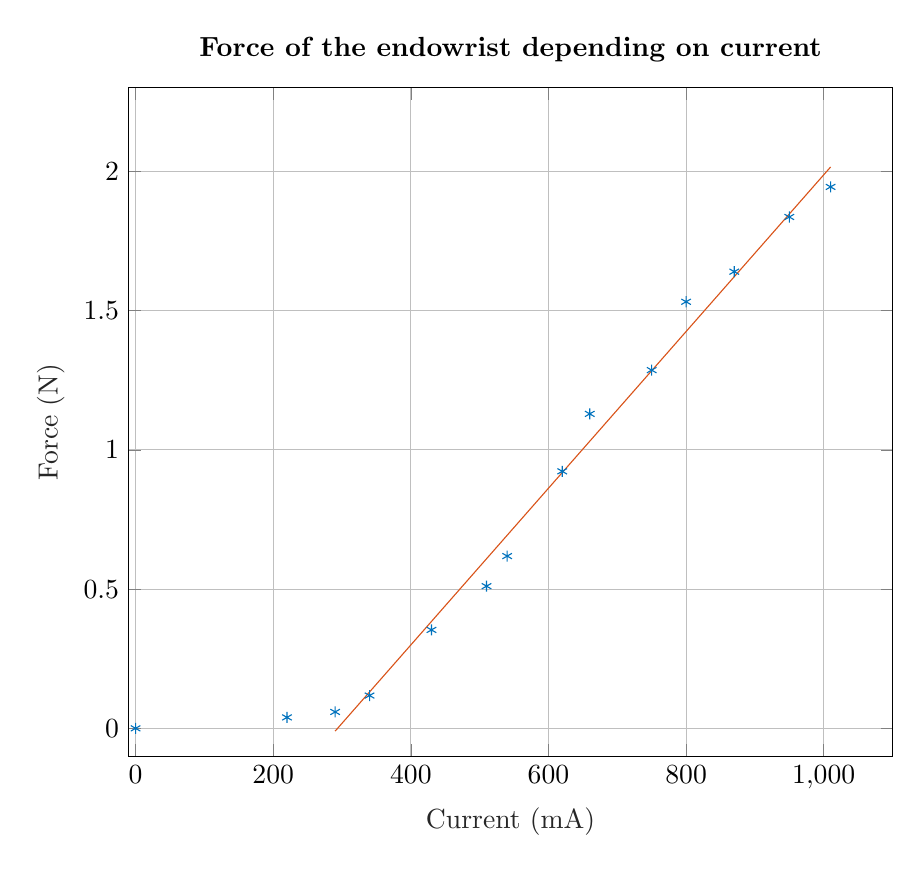
\begin{tikzpicture}

\begin{axis}[%
width=0.8\columnwidth,%7.484in,
height=0.7\columnwidth,%8.26in,
at={(0.758in,0.481in)},
scale only axis,
xmin=-10,
xmax=1100,
xlabel style={font=\color{white!15!black}},
xlabel={Current (mA)},
ymin=-0.1,
ymax=2.3,
ylabel style={font=\color{white!15!black}},
ylabel={Force (N)},
axis background/.style={fill=white},
title style={font=\bfseries},
title={Force of the endowrist depending on current},
xmajorgrids,
ymajorgrids
]
\addplot [color=mycolor1, draw=none, mark=asterisk, mark options={solid, mycolor1}, forget plot]
  table[row sep=crcr]{%
0	0\\
220	0.03928\\
290	0.05892\\
340	0.11784\\
430	0.35352\\
510	0.51064\\
540	0.61866\\
620	0.92308\\
660	1.1293\\
750	1.28642\\
800	1.53192\\
870	1.63994\\
950	1.83634\\
1010	1.94436\\
};
\addplot [color=mycolor2, forget plot]
  table[row sep=crcr]{%
290	-0.00996204344902341\\
340	0.130719594329395\\
430	0.383946542330548\\
510	0.609037162776017\\
540	0.693446145443068\\
620	0.918536765888537\\
660	1.03108207611127\\
750	1.28430902411242\\
800	1.42499066189084\\
870	1.62194495478063\\
950	1.8470355752261\\
1010	2.0158535405602\\
};
\end{axis}
\end{tikzpicture}%
\caption{The force measurements from the end-effector}
\label{endo_force_mes}
\end{figure}

\subsection*{Uncertainties of measurement:}
\begin{itemize}
\item Not 100 \% orthogonal force to the load cell.
\item Input/Output impedance of sensors have a $\pm 10 \%$ tolerance.
\item Movement of test setup when force is generated.
\end{itemize}

\subsection*{Conclusion:}
\todo{conclusion}

\subsection{Pitch down and upwards force} % \label{app:...}
This test uses the test setup seen on \figref{fig:pitch_force}. The positive force is defined as a downwards direction on the load-cell, see \figref{fig:mes_up_down}.

\begin{figure}[H]
	\centering
	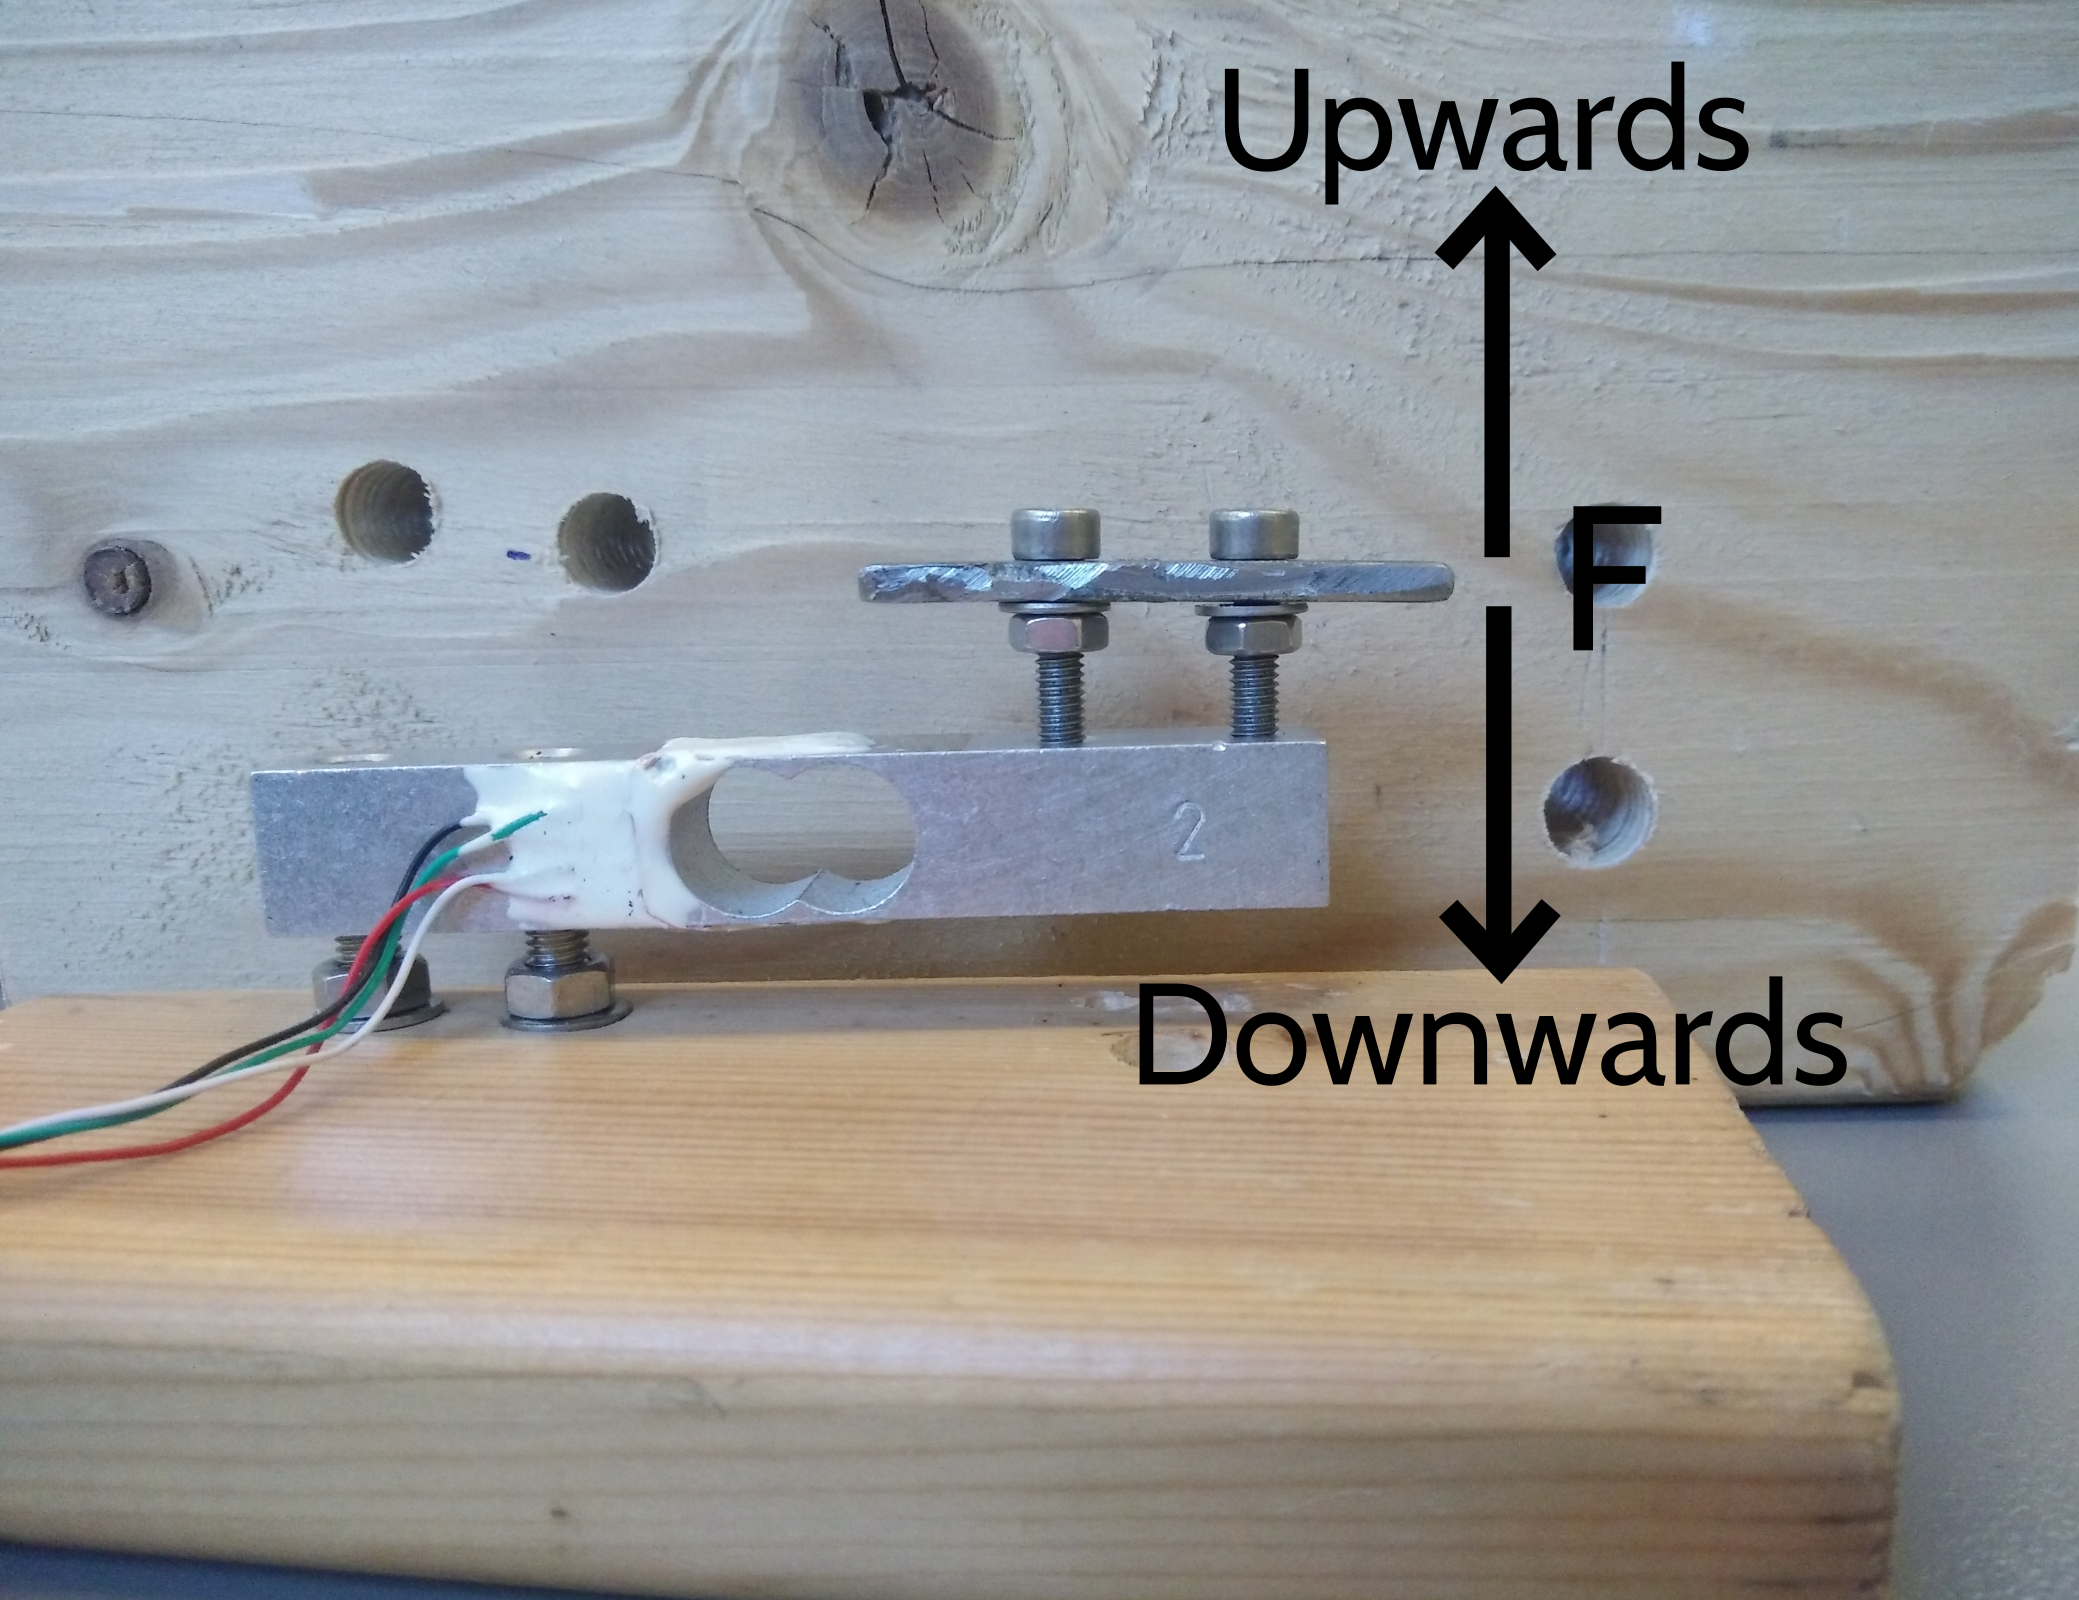
\includegraphics[width=0.4\linewidth]{load_cell_mes.png}
	\caption{Load-cell with defined upwards- downwars force.}
	\label{fig:mes_up_down}
\end{figure}


\subsection*{Test equipment:}
\begin{itemize}
\item Endowrist model 420093 (AAU number: \#4).
\item Maxon 110160 motor with attached Maxon gearhead 110356 and Maxon encoder 201937.
\item Load cell rate for 1 kg of force \cite{Load_cell_1kg}.
\item HX711 - Load cell amplifier \cite{HX711}.
\item Arduino uno with Max351 DAC.
\item sbRIO board.
\end{itemize}

\subsection*{Procedure:}
The following procedure was made:\\
Downwards force measurements:
\begin{enumerate}
\item The end-effector is attached perpendicular to the load cell. 
\item The load cell is reset to zero.
\item Current is applied to the motor which control the pitch of the end-effector, at different current levels and the force is measured (downwards direction).
\item Current is increased until 680 mA is applied.
\end{enumerate}
Step two to four is repeated five times, where the current and force is measured in respect to each other. 

Upwards force measurements:
\begin{enumerate}
\item The end-effector is attached perpendicular to the load cell. 
\item The load cell is reset to zero.
\item Current is applied to the motor which control the pitch of the end-effector, at different current levels and the force is measured (upwards direction).
\item Current is increased until 680 mA is applied.
\end{enumerate}
Step two to four is repeated five times, where the current and force is measured in respect to each other. 

\subsection*{Measuring data:}
Six of the data measurements can be seen on \figref{fig:pitch_down} and \figref{fig:pitch_up}.

\begin{figure}[H]
\centering
\input{Data/Measurement/EndoWrist_Measurements/Force/pitch_down}
\caption{Force measurements for the pitch in an downwards direction.}
\label{fig:pitch_down}
\end{figure}

\begin{figure}[H]
\centering
\input{Data/Measurement/EndoWrist_Measurements/Force/pitch_up}
\caption{Force measurements for the pitch in an upwards direction.}
\label{fig:pitch_up}
\end{figure}

%\figref{endo_force_mes}. 
%\eqref{eq:linear_force_endo}.

% \begin{equation}
% \text{y} = 0.0028 \cdot \text{x} -0.8259 
% \label{eq:linear_force_endo}
% \end{equation} 



\subsection*{Results:}
From \figref{fig:pitch_down} and \figref{fig:pitch_up} a similar pattern between the measurements can be seen. From each measurement it can be seen that the force growth for the different measurements are similar. Force is generated on the end-effector from almost the same current start point on both downwards and upwards measurements. For downwards the force is applied between -131 mA to -148 mA and upwards between 151 mA to 191 mA. It can be seen that the current is decreasing for each measurements. This is due to the controller implemented on the motor controller as it gets a setpoint and current is applied until the setpoint is reached and then decreased.
%It can be seen from the graph on \figref{endo_force_mes} that the force on the end-effector is highly nonlinear. The friction from the gearing and the Endowrist does that the force first has an exponential growth at the start. Around the 800 mA and 1200 mA step it can be seen that a drop in force is happening. What causes this drop is not identified but it can be seen that it appears for all the data sequences. \todor{better explanation?}


%% This file was created by matlab2tikz.
%
%The latest updates can be retrieved from
%  http://www.mathworks.com/matlabcentral/fileexchange/22022-matlab2tikz-matlab2tikz
%where you can also make suggestions and rate matlab2tikz.
%
\definecolor{mycolor1}{rgb}{0.00000,0.44700,0.74100}%
\definecolor{mycolor2}{rgb}{0.85000,0.32500,0.09800}%
%
\begin{figure}[h]
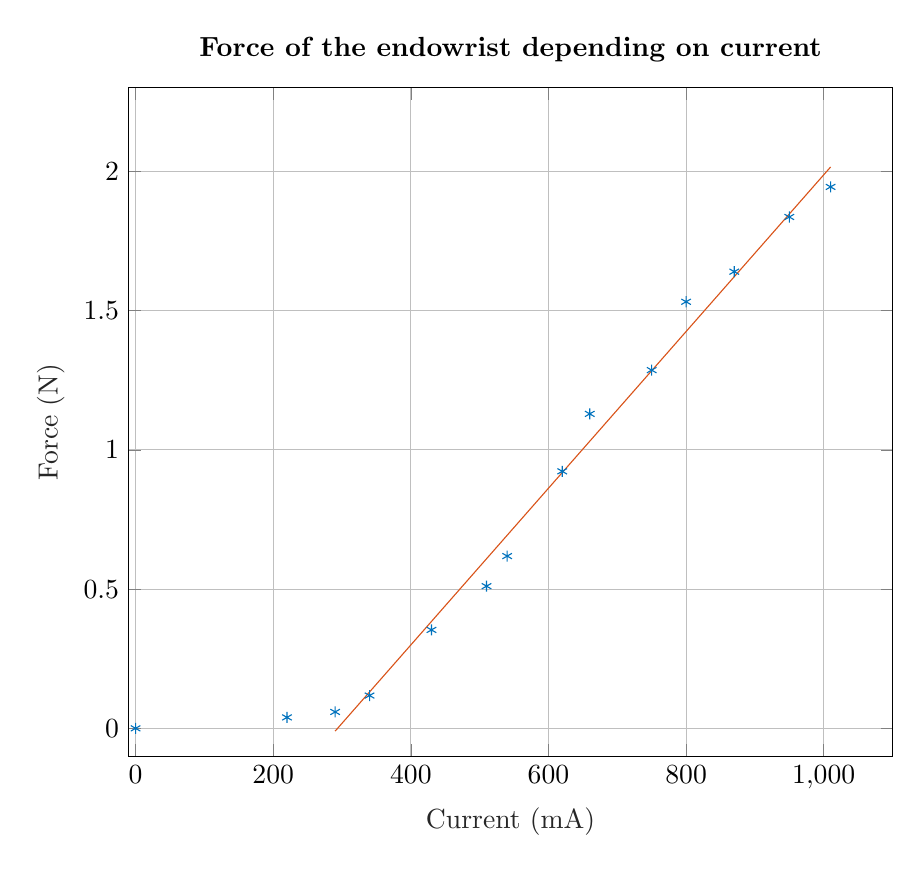
\begin{tikzpicture}

\begin{axis}[%
width=0.8\columnwidth,%7.484in,
height=0.7\columnwidth,%8.26in,
at={(0.758in,0.481in)},
scale only axis,
xmin=-10,
xmax=1100,
xlabel style={font=\color{white!15!black}},
xlabel={Current (mA)},
ymin=-0.1,
ymax=2.3,
ylabel style={font=\color{white!15!black}},
ylabel={Force (N)},
axis background/.style={fill=white},
title style={font=\bfseries},
title={Force of the endowrist depending on current},
xmajorgrids,
ymajorgrids
]
\addplot [color=mycolor1, draw=none, mark=asterisk, mark options={solid, mycolor1}, forget plot]
  table[row sep=crcr]{%
0	0\\
220	0.03928\\
290	0.05892\\
340	0.11784\\
430	0.35352\\
510	0.51064\\
540	0.61866\\
620	0.92308\\
660	1.1293\\
750	1.28642\\
800	1.53192\\
870	1.63994\\
950	1.83634\\
1010	1.94436\\
};
\addplot [color=mycolor2, forget plot]
  table[row sep=crcr]{%
290	-0.00996204344902341\\
340	0.130719594329395\\
430	0.383946542330548\\
510	0.609037162776017\\
540	0.693446145443068\\
620	0.918536765888537\\
660	1.03108207611127\\
750	1.28430902411242\\
800	1.42499066189084\\
870	1.62194495478063\\
950	1.8470355752261\\
1010	2.0158535405602\\
};
\end{axis}
\end{tikzpicture}%
\caption{The force measurements from the end-effector}
\label{endo_force_mes}
\end{figure}
\subsection*{Uncertainties of measurement:}
\begin{itemize}
\item The force applied is not perfectly orthogonal force to the load cell.
\item Input/Output impedance of load-cell sensors have a $\pm 10 \%$ tolerance.
\item Movement of test setup when force is generated.
\end{itemize}

\subsection*{Conclusion:}
Force is generated at the end-effector when a current higher than -131 mA for downwards force and 151 mA for upwards.

%\subsection{Pitch push} % \label{app:...}
This test uses the test setup seen on \figref{fig:pitch_force}.

\subsection*{Test equipment:}
\begin{itemize}
\item Endowrist model 420093 (AAU number: \#4).
\item Maxon 110160 motor with attached Maxon gearhead 110356 and Maxon encoder 201937.
\item Load cell rate for 1 kg of force \cite{Load_cell_1kg}.
\item HX711 - Load cell amplifier \cite{HX711}
\end{itemize}

\subsection*{Procedure:}
The following procedure was made for the push force measurements:
\begin{enumerate}
\item The end-effector is rotated $90^\circ$ and attached perpendicular to the load cell. 
\item The scale is reset to zero.
\item Current is applied to the motor which control the pitch of the end-effector, with different current steps and the force is measured (downwards direction).
\item Current is increased until 1200 mA is applied.
\end{enumerate}
Step two to four is repeated five times, where the current and force is measured in respect to each other. 

\subsection*{Measuring data:}
The data from the measurements can be seen on \todo{Picture}%\figref{endo_force_mes}. 
%\eqref{eq:linear_force_endo}.

% \begin{equation}
% \text{y} = 0.0028 \cdot \text{x} -0.8259 
% \label{eq:linear_force_endo}
% \end{equation} 



\subsection*{Results:}
\todo{result}
%It can be seen from the graph on \figref{endo_force_mes} that the force on the end-effector is highly nonlinear. The friction from the gearing and the Endowrist does that the force first has an exponential growth at the start. Around the 800 mA and 1200 mA step it can be seen that a drop in force is happening. What causes this drop is not identified but it can be seen that it appears for all the data sequences. \todor{better explanation?}


%% This file was created by matlab2tikz.
%
%The latest updates can be retrieved from
%  http://www.mathworks.com/matlabcentral/fileexchange/22022-matlab2tikz-matlab2tikz
%where you can also make suggestions and rate matlab2tikz.
%
\definecolor{mycolor1}{rgb}{0.00000,0.44700,0.74100}%
\definecolor{mycolor2}{rgb}{0.85000,0.32500,0.09800}%
%
\begin{figure}[h]
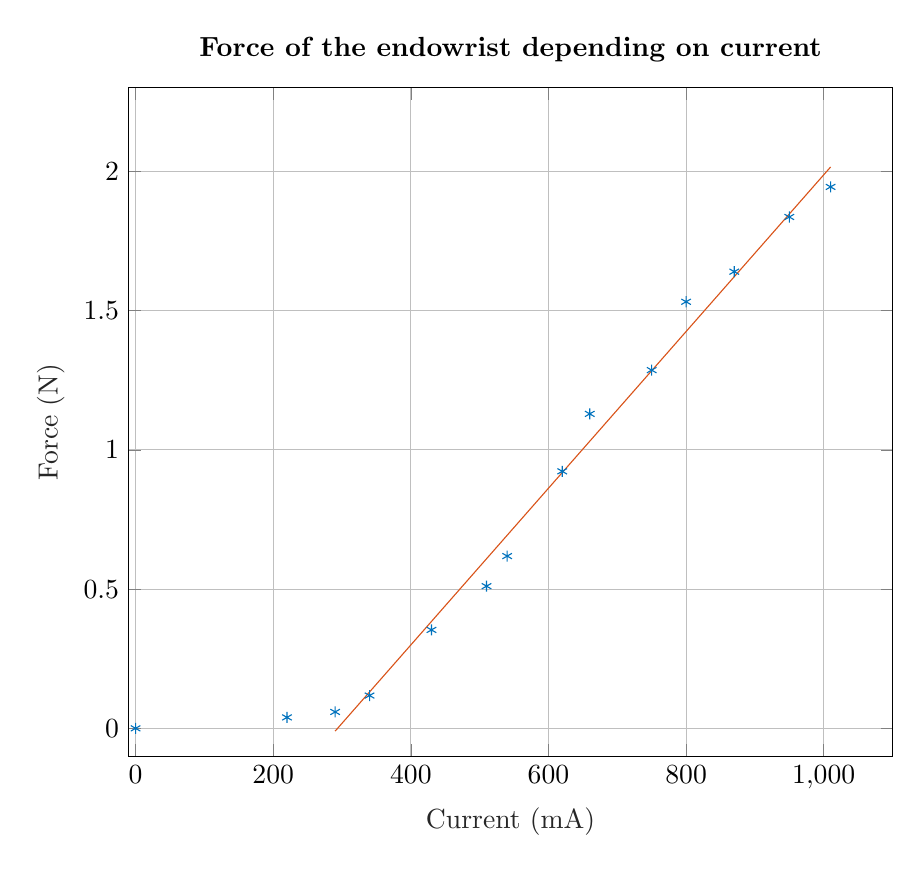
\begin{tikzpicture}

\begin{axis}[%
width=0.8\columnwidth,%7.484in,
height=0.7\columnwidth,%8.26in,
at={(0.758in,0.481in)},
scale only axis,
xmin=-10,
xmax=1100,
xlabel style={font=\color{white!15!black}},
xlabel={Current (mA)},
ymin=-0.1,
ymax=2.3,
ylabel style={font=\color{white!15!black}},
ylabel={Force (N)},
axis background/.style={fill=white},
title style={font=\bfseries},
title={Force of the endowrist depending on current},
xmajorgrids,
ymajorgrids
]
\addplot [color=mycolor1, draw=none, mark=asterisk, mark options={solid, mycolor1}, forget plot]
  table[row sep=crcr]{%
0	0\\
220	0.03928\\
290	0.05892\\
340	0.11784\\
430	0.35352\\
510	0.51064\\
540	0.61866\\
620	0.92308\\
660	1.1293\\
750	1.28642\\
800	1.53192\\
870	1.63994\\
950	1.83634\\
1010	1.94436\\
};
\addplot [color=mycolor2, forget plot]
  table[row sep=crcr]{%
290	-0.00996204344902341\\
340	0.130719594329395\\
430	0.383946542330548\\
510	0.609037162776017\\
540	0.693446145443068\\
620	0.918536765888537\\
660	1.03108207611127\\
750	1.28430902411242\\
800	1.42499066189084\\
870	1.62194495478063\\
950	1.8470355752261\\
1010	2.0158535405602\\
};
\end{axis}
\end{tikzpicture}%
\caption{The force measurements from the end-effector}
\label{endo_force_mes}
\end{figure}

\subsection*{Uncertainties of measurement:}
\begin{itemize}
\item Not 100 \% orthogonal force to the load cell.
\item Input/Output impedance of sensors have a $\pm 10 \%$ tolerance.
\item Movement of test setup when force is generated.
\end{itemize}

\subsection*{Conclusion:}
\todo{conclusion}

\subsection{EndoWrist roll measurement}% \label{app:...}
The test setup for this measurement can be seen on \todo{figref and a picture below}

\subsection*{Test equipment:}
\begin{itemize}
\item Endowrist model 420093 (AAU number: \#4).
\item Maxon 110160 motor with attached Maxon gearhead 110356 and Maxon encoder 201937.
\item Torque sensor - Holger clasen: MWA-W8-1-P (AAU number: LBNR 08931).
\item Active low pass filter set to 100 Hz and gain 1 (AAU number: C2-104-H1).
\item Agilent 54621A oscilloscope (AAU number: 56684)
\end{itemize}

\subsection*{Procedure:}
The following procedure was made for the push force measurements:
\begin{enumerate}
\item The carbon stick of the EndoWrist is attached to the torque sensor. 
\item The torque sensor is connected to the low pass filter and the low pass filter to the oscilloscope.
\item Current is applied or increased to the motor which control the roll of the end-effector, with different current steps and the output from the torque sensor is noted.
\item Current is increased until 1200 mA is applied.
\end{enumerate}
Step three and four is repeated four times, where the current and torque is noted in respect to each other.. 
\todo{update n times}

\subsection*{Measuring data:}
The data from the measurements can be seen on \figref{fig_roll_mes}

\begin{figure}
% This file was created by matlab2tikz.
%
%The latest updates can be retrieved from
%  http://www.mathworks.com/matlabcentral/fileexchange/22022-matlab2tikz-matlab2tikz
%where you can also make suggestions and rate matlab2tikz.
%
\definecolor{mycolor1}{rgb}{0.00000,0.44700,0.74100}%
\definecolor{mycolor2}{rgb}{0.85000,0.32500,0.09800}%
\definecolor{mycolor3}{rgb}{0.92900,0.69400,0.12500}%
\definecolor{mycolor4}{rgb}{0.49400,0.18400,0.55600}%
%
\begin{figure}
\begin{tikzpicture}

\begin{axis}[%
width=4.521in,
height=3.566in,
at={(0.758in,0.481in)},
scale only axis,
xmin=0,
xmax=1.2,
xlabel style={font=\color{white!15!black}},
xlabel={Curremt [A]},
ymin=0,
ymax=9,
ylabel style={font=\color{white!15!black}},
ylabel={Torque [Ncm]},
axis background/.style={fill=white},
title style={font=\bfseries},
title={Relation between roll force and ampere}
]
\addplot [color=mycolor1, draw=none, mark=asterisk, mark options={solid, mycolor1}, forget plot]
  table[row sep=crcr]{%
0.063	0.34\\
0.097	0.4\\
0.125	0.6\\
0.16	0.8\\
0.208	1.1\\
0.241	1.32\\
0.3	1.86\\
0.38	2.1\\
0.73	4.7\\
1.02	6.68\\
};
\addplot [color=mycolor2, draw=none, mark=asterisk, mark options={solid, mycolor2}, forget plot]
  table[row sep=crcr]{%
0.06	0.7\\
0.12	0.72\\
0.175	0.9\\
0.24	1.54\\
0.3	2\\
0.37	2.42\\
0.42	2.88\\
0.489	3.26\\
0.568	4\\
0.73	4.98\\
0.876	6\\
1.12	7.5\\
};
\addplot [color=mycolor3, draw=none, mark=asterisk, mark options={solid, mycolor3}, forget plot]
  table[row sep=crcr]{%
0.03	0.04\\
0.06	0.8\\
0.276	2.02\\
0.42	3.06\\
0.568	4.24\\
0.73	5.24\\
0.877	6.48\\
1.02	7.28\\
};
\addplot [color=mycolor4, draw=none, mark=asterisk, mark options={solid, mycolor4}, forget plot]
  table[row sep=crcr]{%
0.064	1.2\\
0.16	1.38\\
0.275	2.12\\
0.389	2.86\\
0.51	3.84\\
0.631	4.82\\
0.78	5.7\\
0.94	7.06\\
1.12	8.1\\
};
\end{axis}
\end{tikzpicture}%
\caption{Torque measurements of the roll on the EndoWrist.}
\label{fig:torque_measurement}
\end{figure}
\caption{Torque measurements of the roll on the EndoWrist.}
\label{fig_roll_mes}
\end{figure}
%\figref{endo_force_mes}. 
%\eqref{eq:linear_force_endo}.

% \begin{equation}
% \text{y} = 0.0028 \cdot \text{x} -0.8259 
% \label{eq:linear_force_endo}
% \end{equation} 



\subsection*{Results:}
The measurements shows a similar pattern for each measurements and the torque generated starts under 100 mA for each measurements.


%It can be seen from the graph on \figref{endo_force_mes} that the force on the end-effector is highly nonlinear. The friction from the gearing and the Endowrist does that the force first has an exponential growth at the start. Around the 800 mA and 1200 mA step it can be seen that a drop in force is happening. What causes this drop is not identified but it can be seen that it appears for all the data sequences. \todor{better explanation?}


%% This file was created by matlab2tikz.
%
%The latest updates can be retrieved from
%  http://www.mathworks.com/matlabcentral/fileexchange/22022-matlab2tikz-matlab2tikz
%where you can also make suggestions and rate matlab2tikz.
%
\definecolor{mycolor1}{rgb}{0.00000,0.44700,0.74100}%
\definecolor{mycolor2}{rgb}{0.85000,0.32500,0.09800}%
%
\begin{figure}[h]
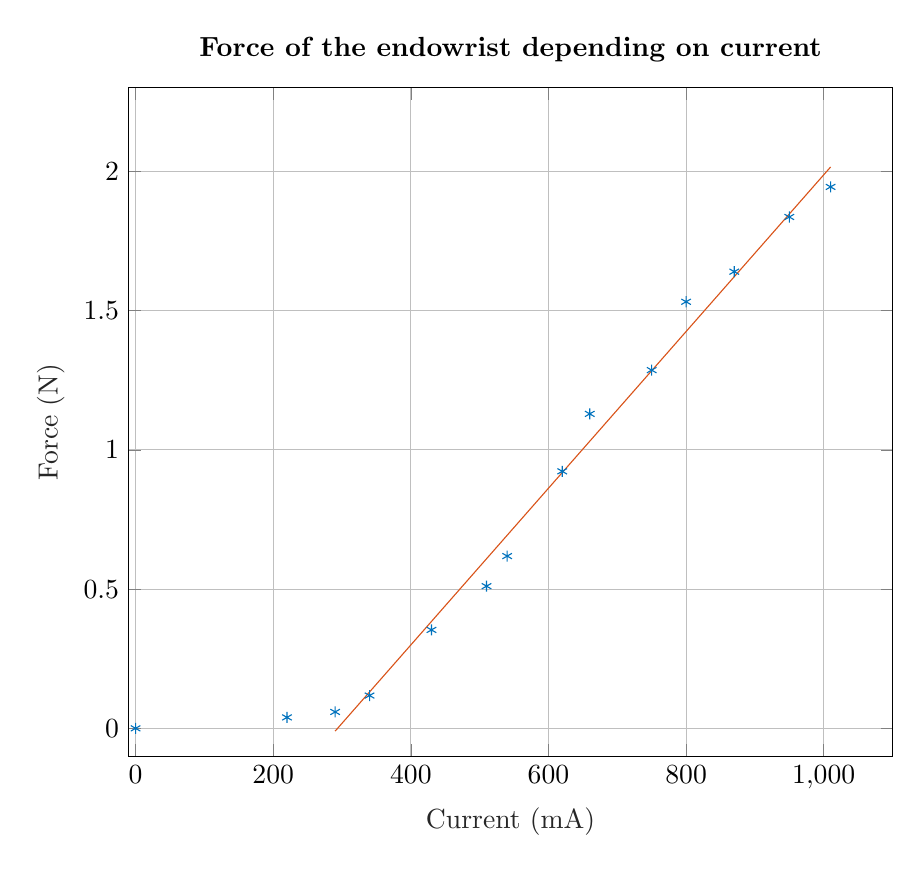
\begin{tikzpicture}

\begin{axis}[%
width=0.8\columnwidth,%7.484in,
height=0.7\columnwidth,%8.26in,
at={(0.758in,0.481in)},
scale only axis,
xmin=-10,
xmax=1100,
xlabel style={font=\color{white!15!black}},
xlabel={Current (mA)},
ymin=-0.1,
ymax=2.3,
ylabel style={font=\color{white!15!black}},
ylabel={Force (N)},
axis background/.style={fill=white},
title style={font=\bfseries},
title={Force of the endowrist depending on current},
xmajorgrids,
ymajorgrids
]
\addplot [color=mycolor1, draw=none, mark=asterisk, mark options={solid, mycolor1}, forget plot]
  table[row sep=crcr]{%
0	0\\
220	0.03928\\
290	0.05892\\
340	0.11784\\
430	0.35352\\
510	0.51064\\
540	0.61866\\
620	0.92308\\
660	1.1293\\
750	1.28642\\
800	1.53192\\
870	1.63994\\
950	1.83634\\
1010	1.94436\\
};
\addplot [color=mycolor2, forget plot]
  table[row sep=crcr]{%
290	-0.00996204344902341\\
340	0.130719594329395\\
430	0.383946542330548\\
510	0.609037162776017\\
540	0.693446145443068\\
620	0.918536765888537\\
660	1.03108207611127\\
750	1.28430902411242\\
800	1.42499066189084\\
870	1.62194495478063\\
950	1.8470355752261\\
1010	2.0158535405602\\
};
\end{axis}
\end{tikzpicture}%
\caption{The force measurements from the end-effector}
\label{endo_force_mes}
\end{figure}

\subsection*{Uncertainties of measurement:}
\begin{itemize}
\item Gain of low pass filter could deviate from 1.
\item Noise did still appear after the filter and could affect the output reading.
\end{itemize}

\subsection*{Conclusion:}
It can be seen on figure \figref{fig_roll_mes} that the roll-torque of the EndoWrist has a linear growth from under approx 100 mA and up.






% \begin{figure}[H]
% 	\centering
% 	\begin{subfigure}{.45\textwidth}
% 		\centering
% 		\vspace{24pt}
% 		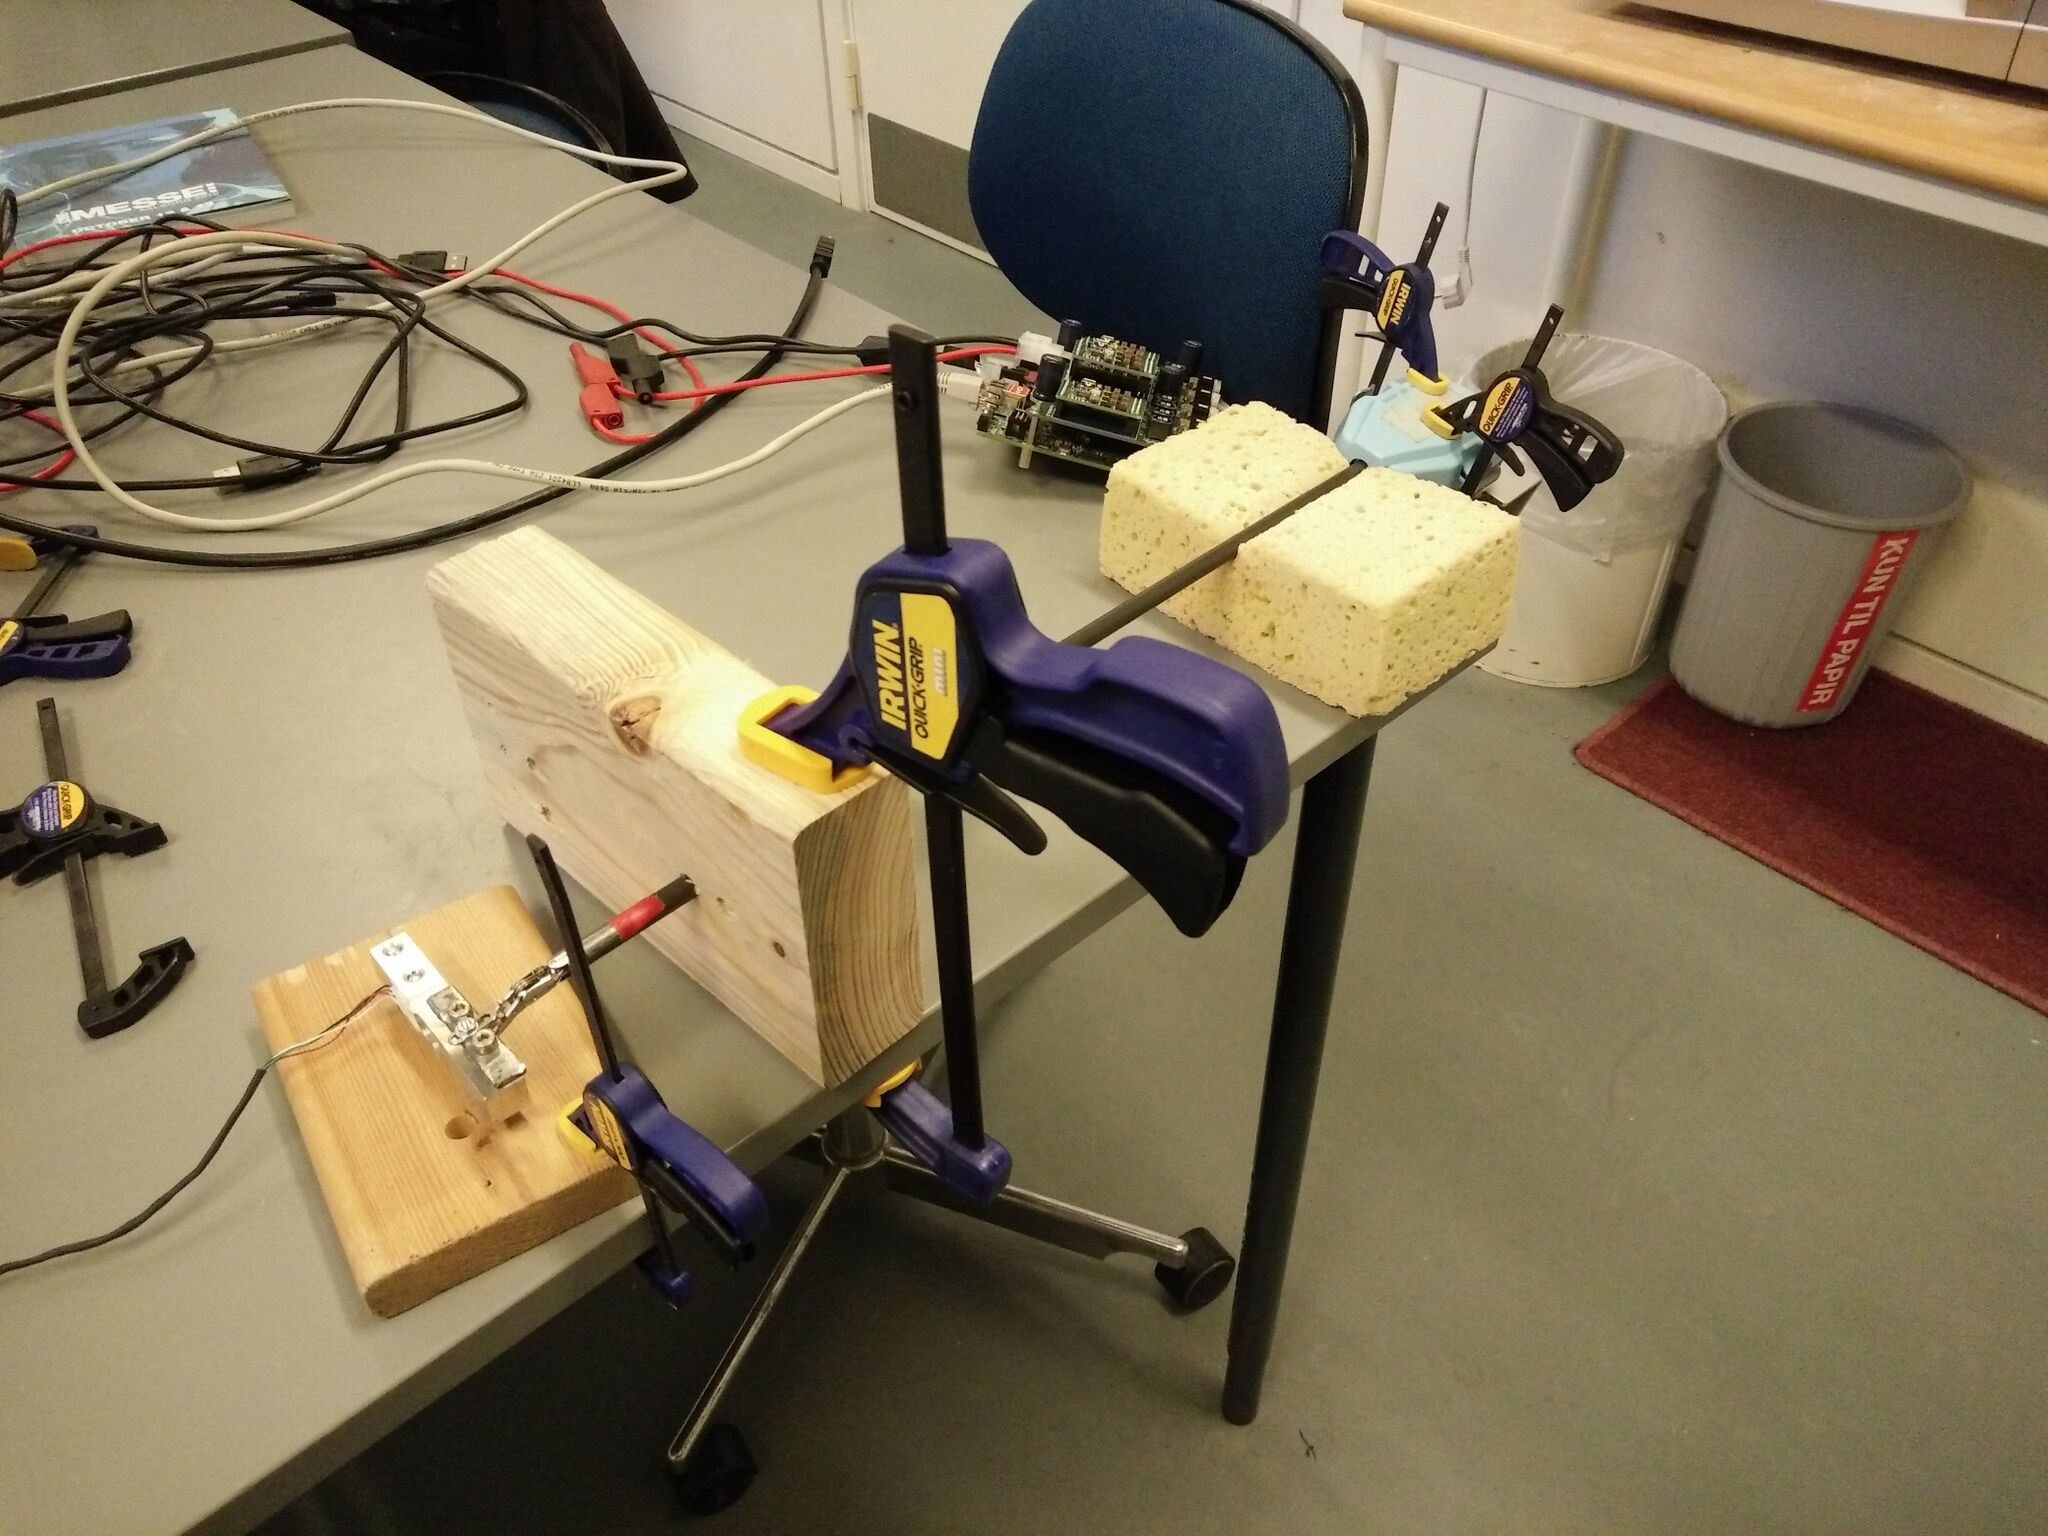
\includegraphics[width=\linewidth]{overall_force.jpg}
% 		\caption{The entire test setup. From the right, a load cell for measuring the downwards force, a piece of wood for stiffening the Endowrist and keeping it it place and the Endowrist holder with motors.}
% 		\label{fig:entire_force_testsetup}
% 	\end{subfigure}
% 	\begin{subfigure}{.45\textwidth}
% 		\centering
% 		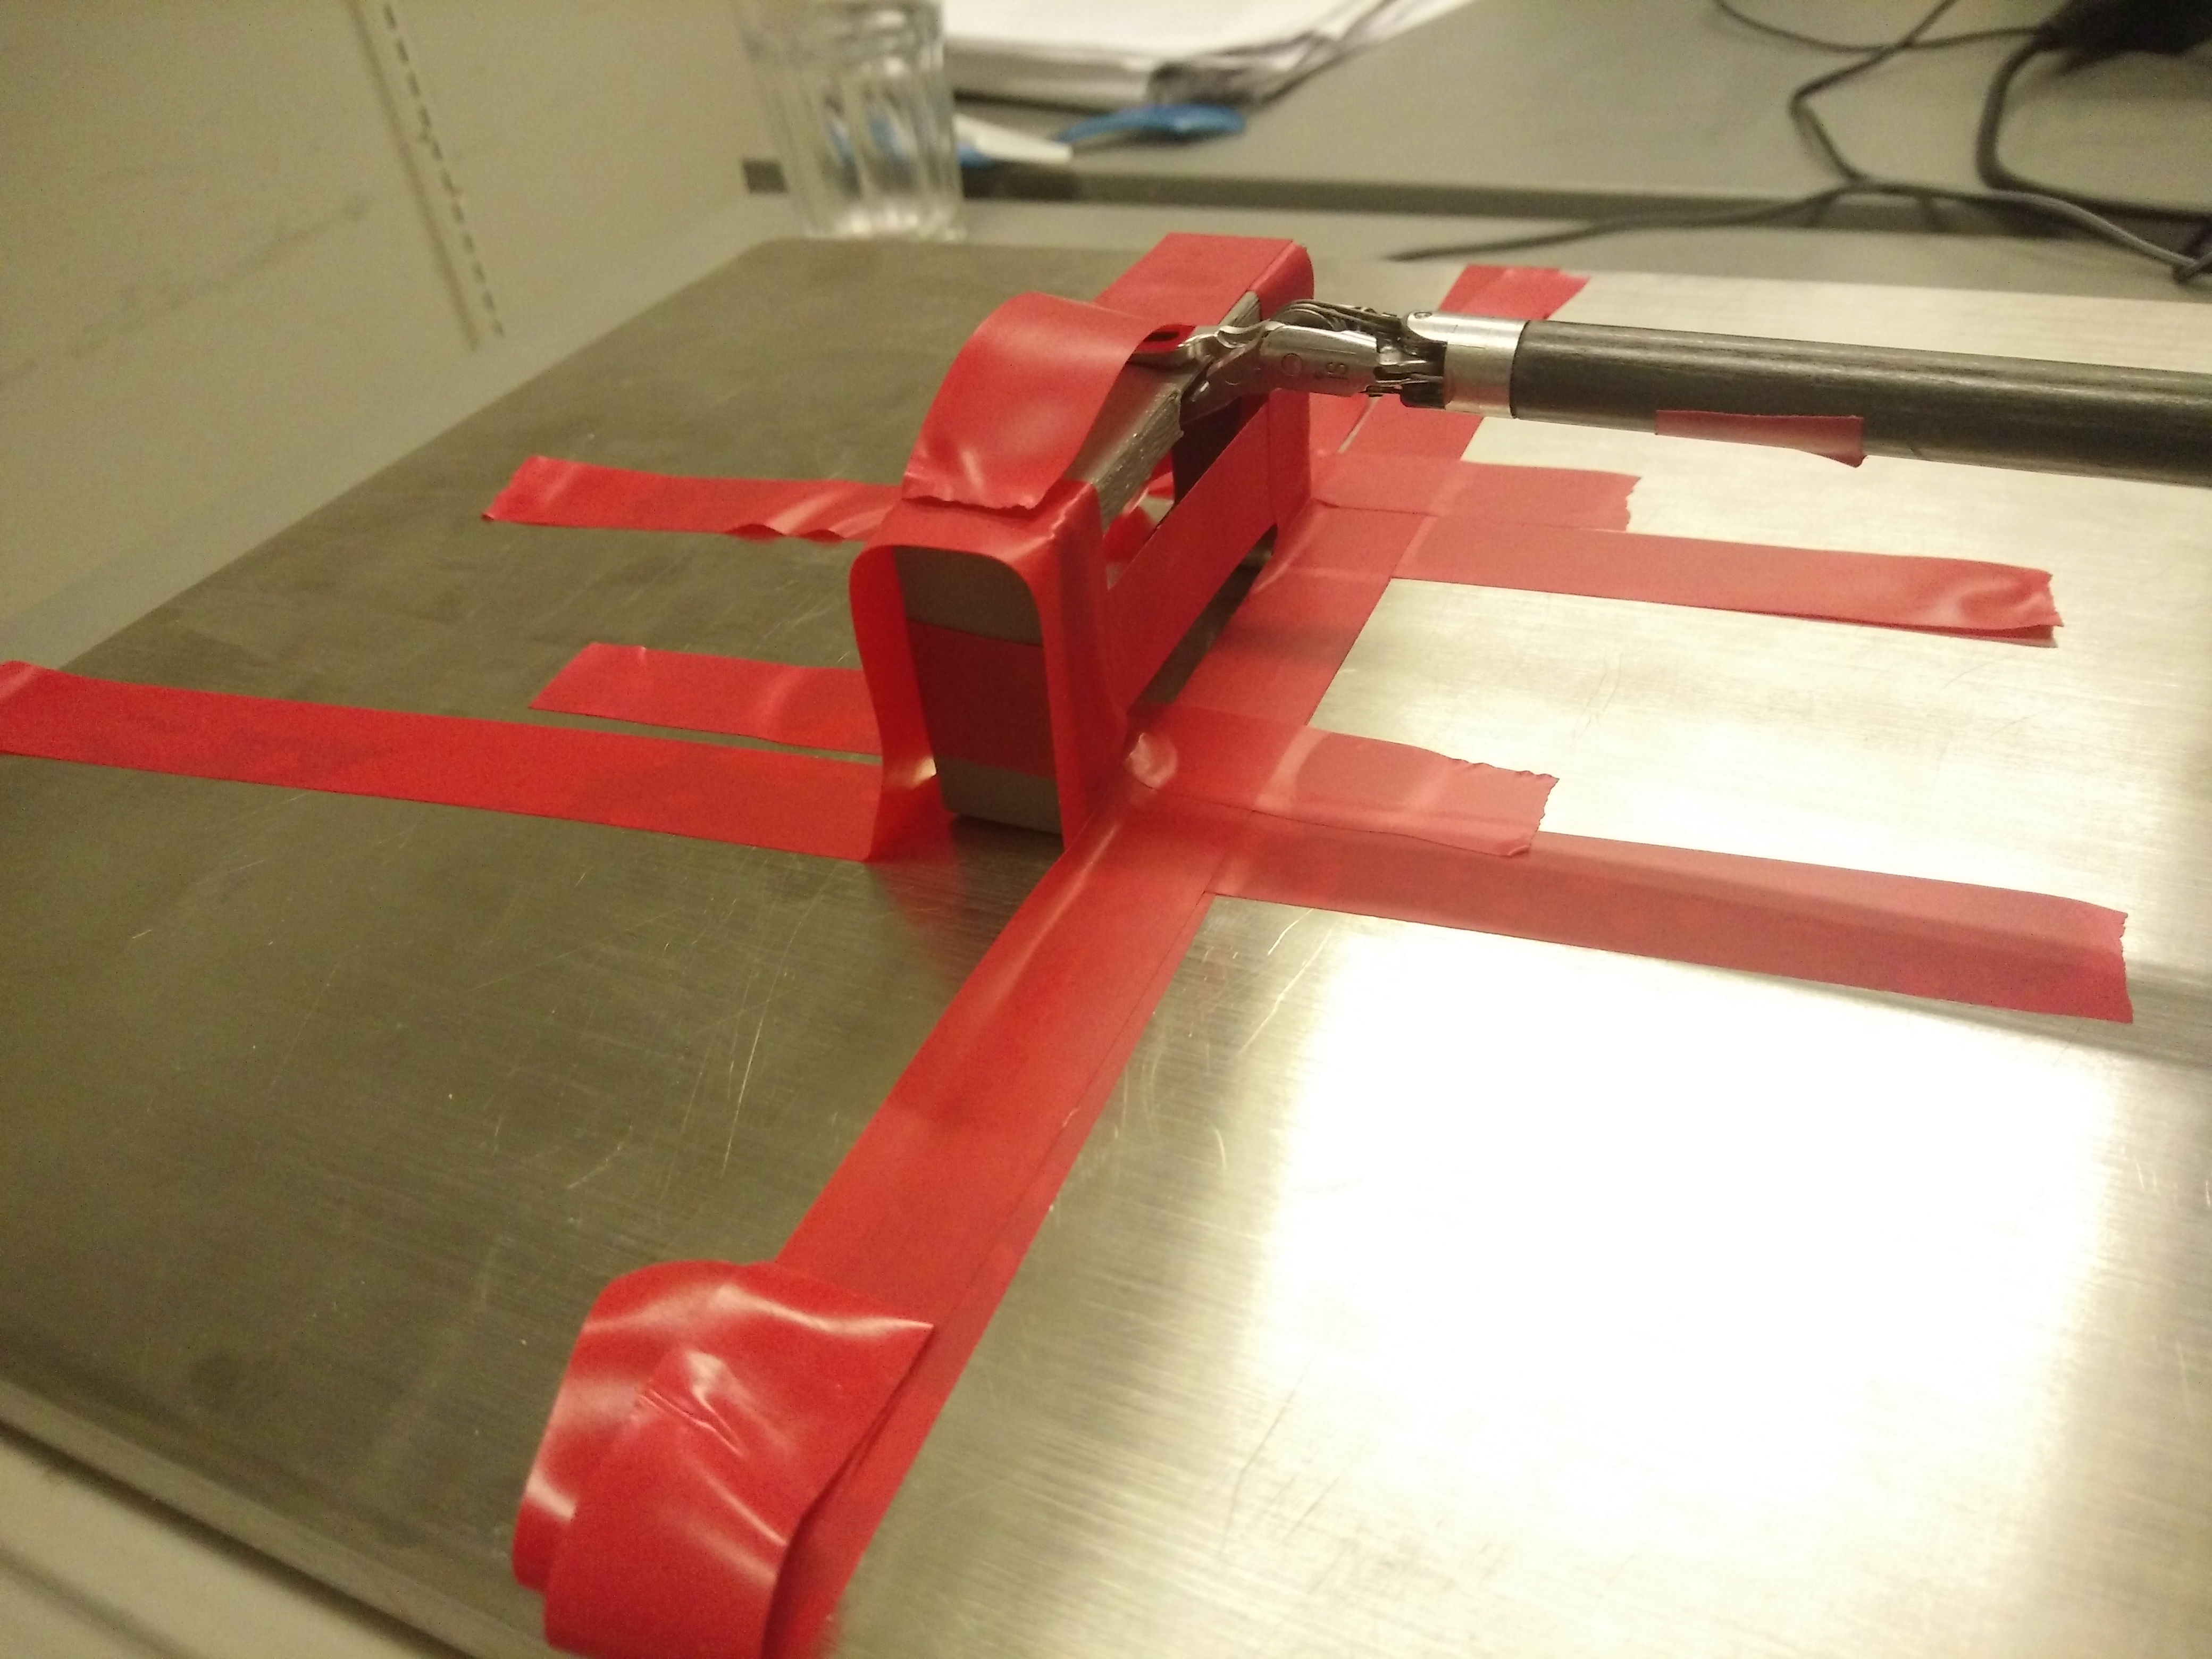
\includegraphics[width=\linewidth]{endeffector_force.jpg}
% 		\caption{The load cell with the attached end-effector.}
% 		\label{fig:endeffector_force}
% 	\end{subfigure}
% \caption{Test setup for the force estimation of the end-effector.}
% \label{fig:Overview_force}
% \end{figure}



